\documentclass[a4paper, 11pt, notitlepage, english]{article}

\usepackage{babel}
\usepackage[utf8]{inputenc}
\usepackage[T1]{fontenc, url}
\usepackage{textcomp}
\usepackage{amsmath, amssymb}
\usepackage{amsbsy, amsfonts}
\usepackage{graphicx, color}
\usepackage{parskip}
\usepackage{framed}
\usepackage{amsmath}
\usepackage[table]{xcolor}
\usepackage{multicol}
\usepackage{url}
\usepackage{flafter}


\usepackage{geometry}
\geometry{headheight=0.01mm}
\geometry{top=24mm, bottom=29mm, left=39mm, right=39mm}

\renewcommand{\arraystretch}{2}
\setlength{\tabcolsep}{10pt}
\makeatletter
\renewcommand*\env@matrix[1][*\c@MaxMatrixCols c]{%
  \hskip -\arraycolsep
  \let\@ifnextchar\new@ifnextchar
  \array{#1}}
%
% Parametere for inkludering av kode fra fil
%
\usepackage{listings}
\lstset{language=python}
\lstset{basicstyle=\ttfamily\small}
\lstset{frame=single}
\lstset{keywordstyle=\color{red}\bfseries}
\lstset{commentstyle=\itshape\color{blue}}
\lstset{showspaces=false}
\lstset{showstringspaces=false}
\lstset{showtabs=false}
\lstset{breaklines}

%
% Definering av egne kommandoer og miljøer
%
\newcommand{\dd}[1]{\ \text{d}#1}
\newcommand{\f}[2]{\frac{#1}{#2}} 
\newcommand{\beq}{\begin{equation}}
\newcommand{\eeq}{\end{equation}}
\newcommand{\bra}[1]{\langle #1|}
\newcommand{\ket}[1]{|#1 \rangle}
\newcommand{\braket}[2]{\langle #1 | #2 \rangle}
\newcommand{\braup}[1]{\langle #1 \left|\uparrow\rangle\right.}
\newcommand{\bradown}[1]{\langle #1 \left|\downarrow\rangle\right.}
\newcommand{\av}[1]{\left| #1 \right|}
\newcommand{\op}[1]{\hat{#1}}
\newcommand{\braopket}[3]{\langle #1 | {#2} | #3 \rangle}
\newcommand{\ketbra}[2]{\ket{#1}\bra{#2}}
\newcommand{\pp}[1]{\frac{\partial}{\partial #1}}
\newcommand{\ppn}[1]{\frac{\partial^2}{\partial #1^2}}
\newcommand{\up}{\left|\uparrow\rangle\right.}
\newcommand{\upup}{\left|\uparrow\uparrow\rangle\right.}
\newcommand{\down}{\left|\downarrow\rangle\right.}
\newcommand{\downdown}{\left|\downarrow\downarrow\rangle\right.}
\newcommand{\updown}{\left|\uparrow\downarrow\rangle\right.}
\newcommand{\downup}{\left|\downarrow\uparrow\rangle\right.}
\newcommand{\bupup}{\left.\langle\uparrow\uparrow\right|}
\newcommand{\bdowndown}{\left.\langle\downarrow\downarrow\right|}
\newcommand{\bupdown}{\left.\langle\uparrow\downarrow\right|}
\newcommand{\bdownup}{\left.\langle\downarrow\uparrow\right|}
\renewcommand{\d}{{\rm d}}
\renewcommand{\b}{\bigg}
\newcommand{\Res}[2]{{\rm Res}(#1;#2)}
\newcommand{\To}{\quad\Rightarrow\quad}
\newcommand{\eps}{\epsilon}
\newcommand{\inner}[2]{\langle #1 , #2 \rangle}

\renewcommand{\up}{\uparrow}
\renewcommand{\down}{\downarrow}

\newcommand{\bt}[1]{\boldsymbol{#1}}
\newcommand{\mat}[1]{\textsf{\textbf{#1}}}
\newcommand{\I}{\boldsymbol{\mathcal{I}}}
\newcommand{\p}{\partial}
%
% Navn og tittel
%
\author{}
\title{Notes in FYS4130---Statistical physics}


\begin{document}

%%%%%%%%%%%%%%%%%%%%%%%%%%%%%%%%%%%%%%%%%%%%%%%%%%%%%%%%
%%%%%%%%%%%%%%%%%%%%%%%%%%%%%%%%%%%%%%%%%%%%%%%%%%%%%%%%
%%%%%%                                            %%%%%%
%%%%%%              MOLECULAR DYNAMICS            %%%%%%
%%%%%%                                            %%%%%%
%%%%%%%%%%%%%%%%%%%%%%%%%%%%%%%%%%%%%%%%%%%%%%%%%%%%%%%%
%%%%%%%%%%%%%%%%%%%%%%%%%%%%%%%%%%%%%%%%%%%%%%%%%%%%%%%%



%%%%%%%%%%%%%%%%%%%%
%%%  QUESTION 1  %%%
%%%%%%%%%%%%%%%%%%%%

\section{Molecular-dynamics algorithms}

Discuss the algorithms for molecular-dynamics modeling:
\begin{itemize}
	\item Potentials
	\item Integration
	\item Cut-off
	\item Periodic boundary Conditions
	\item Initialization
	\item Efficiency improvements
\end{itemize}

\subsubsection*{Potentials}

The potential function is the most crucial part, as it is what defines the interaction between the particles. Some potentials are defined between pair of particles, so called two-body potentials. Sometimes we invoke three-body or many-body potentials.

A good example of a two-body potential is the Leonnard-Jones potential, aka the 6--12 potential.
$$U(r) = 4\eps \bigg[\b(\frac{r}{\sigma}\b)^{12} - \b(\frac{r}{\sigma}\b)^6\bigg].$$
The $\eps$ and $\sigma$ are parameters that can be fitted to simulate different gases. In principle, the LJ-potential is used to simulate noble gases, as covalent and metallic bonding is more complex. The $\eps$ paramter gives the `strength' of the force, and the $\sigma$ gives the length scale. The 12-term describes Pauli repulsion, the 6-term describes dipole-dipole attraction (van der Waal-force).

Most practical potentials are specially constructed/fitted to be specific to a given problem/system. For example, the \textbf{Weber-Stillinger} potential is made to describe silicon. In equilibrium silicon aligns in tetrhedral structures with tight bonds. A spherical symmetrical potential cannot caputre this behaviour in a meaningful way. The W-S potential does it by combining a two-body and a three-body contribution. The three-body part describes the bedning stiffness of the system and the two-body part is L-J like.


\subsubsection*{Integration}

It is very common to use the velocity-verlet method to integrate Newton's equations of motion. It is effectively a leap-frog method without a staggered grid, meaning the velocity equation is solved using the midpoint method in position and vice versa. In practice, this is done by computing the velocity in two half-steps. The velocity-verlet is therefore sometimes called half-kick/drift/half-kick. So we have
\begin{align*}
v_{i + 1/2} &= v_i + a_i \frac{\Delta t}{2}, \\
x_{i+1} &= x_i + v_{i+1/2}\Delta t, \\
v_{i + 1} &= v_{i + 1/2} + a_{i+1} \frac{\Delta t}{2}.
\end{align*}
Note that to perform the last step, the acceleration must first be evaluated from $a_{i+1} = -\d U(x_{i+1}) / \d x,$ which is why the velocity uses the midpoint method.

As for the leapfrog method, velocity-verlet is of global order $\mathcal{O}(\Delta^2)$ as it uses the midpoint method to solve the equations of motion per time step, which has the error $\mathcal{O}(\Delta t^3)$, but then we repeat this for $N=T/\Delta t$ steps.

The benefits of velocity-verlet are
\begin{itemize}
	\item Preserves the time-reversability of the equations of motion
	\item Conserves angular momentum exactly for spherical symmetrical potentials
	\item Symplectic, i.e., obeys Liouville's theorem and is area preserving in phase space (this gives them global stability as the energy cannot increase without bound, that would make the area in phase space grow).
	\item Of better order than euler methods, including Euler-Cromer which has global error of $\mathcal{O}(\Delta t)$ (as it is second-order per timestep).
\end{itemize}

However, the velocity-verlet is NOT energy conserving (on short time-scales), which the equations of motions should be! Velocity verlet is usually the preferred version of Verlet integration since it has better precision in finite-precision arithmetic

Now, there are methods with smaller errors, such as RK4, but RK4 is NOT symplectic as the determinant of it's jacobian is not 1, therefore RK4 is very risky to use. It is very accurate, so the energy won't grow quickly, but over long time scales, it might grow beyond any bounds and the entire simulation might collapse.

Now, one might question why not turn to a higher-order symplectic integrators? They do exist, for example the Forest-Ruth algorithm which is time-reversible, symplectic and of global order $\mathcal{O}(\Delta t^4)$, the answer is simply that close enough is good enough combined with computational cost. The Forest-Ruth algorithm requires three force-calculations per step, which are very costly. Algorithms such as PEFRL require 4 force calculations per step, a rough estimate then tells us that we can compare PEFRL with a time step four times larger than that of velocity-verlet, PEFRL still comes out much more accurate.

Which method is best depends on use. In some cases, adaptive schemes might be the best.

\subsubsection*{Cut-off}

The most expensive part of MD simulation computationally is the force calculation. The number of pairs in a system grows as $\mathcal{O}(N^2)$, while the cost of the velocity verlet is $\mathcal{O}(N)$ (if we exclude the force calculation). However, most two-body interactions, such as the LJ potentialare short-ranged, so we can safely ignore many of these force calculations. By looking at the LJ potential, we can see that when $r$ becomes large, $V(r)\approx 0$. We now implement cut-off by defining some distance to big enough, so that we turn $V(r>r_c) = 0$. When we do this, we should shift the entire potential by the constant $V(r_c)$, so that we do not have a discontinious potential.

Now, this means any pair of particles where the distance between them is bigger than $r_c$ can be ignored in the force calculation---the question is just how we do this computationally. If we need to calculate the distance and check, we still have complexity $\mathcal{O}(N^2)$. The answer is neighbor-lists, there are two types: Cell lists, and verlet lists.

In cell lists, we divide the entire system into cubic cells where the width of each box is at least $r_c$. An atom in a given cell then only needs to consider atoms in their own cells and all the neighboring cells. All other particles are more than one cell away, so there is no force. Figuring out which cell each atom belongs to is obviously $\mathcal{O}(N)$ and must be done every time step. When we know what atoms are in each cell, looping over all neighboring atoms can be done in constant time, assuming the particle density $\rho$ is an intensive quantity, i.e., it does not increase with $N$---this is usually a very good assumption. Since we can calculate the force on any given atom in constant time, the overall complexity of a force calculation obviously becomes $\mathcal{O}(N)$.

In verlet lists each atom has a list of pointers to their nearest atoms. Any atom closer than $r_c + \eps$ is listed. Now, making a verlet list costs a lot, but if $\eps$ is big enough, we can do several force calculations before reconstructing a verlet list (unlike cell lists). We can combine the two concepts. Using a cell list, we can create verlet lists cheaper.

For L-J, the cutof is usually taken to be $r_{\rm cut} = 3\sigma$.

\subsubsection*{Periodic Boundary Conditions}

As in any physical problem, we need a set of boundary conditions. There are various posibilities open to us, we could simulate particles in a box (hard walls), in a vacuum (no walls) or periodic boundary conditions (bulk). The particles in a box and vacuum are usually not of that much interest. Due to computational constraints, we cannot really compute for macroscopic quantities of a substance, and so using PBC let us simulate bulk properties of that material without having our results being messed up due to boundary effects.

When we implement periodic boundary conditions, any particle that would leave the box, enters it on the opposite side of the box with its velocity maintained, so that the kinetic energy is maintained. Now, to properly evaluate the potential between pairs of particles, we need to use the minimum image convention. \emph{Images} are the `copies' of the box we are actually simulating, and so the `closest' particle might be in the next image, not neccesairly our box.

PBC leads to conservation of linear momentum, but not angular momentum. This is dubbed the `NVEPG' ensamble or the molecular-dynamics ensamble. It is very close to the micro-cannonical ensamble, but can lead to some small weird artifacts.

\subsubsection*{Initialization}

We also have initial conditions, and we have to be slightly careful with these, however, they are quite forgiving. We usually start out with the atoms a structure grid or lattice. In our project we started of with all the atoms in a face-centered lattice. In addition we give the atoms randomly distributed velocities. What distribution we choose for the velocities will define the total energy of the system. We usually choose a Boltzmann distribution, as this is what we expect the velocities to tend towards anyway. We then eliminate drift by subracting the average velocity from all particles.

When the system is started it \emph{is not} in thermal equilibrium, and there will be drastic changes as the system tends to thermal equilibrium. We call this process equilibriation. If we are going to be looking at a similar system for many different simulation and measurements, we could always store the state of the system after equilibriating it, meaning we can initialize or system very close to a thermal equilibrium in the future.

An important consideration is that the average particle density cannot change within a given simulation (unless of course we change the size of the PBC slowly over time steps), so we should initialize the system with a particle density close to the phase we want to study. If we want to study the gas phase, we shouldn't start the system of as compactly as a solid, as the system has noe room to expand.

Thermostats can be used to bring the system to a target temperature, then turned of.

\subsubsection*{Efficiency improvements}

The cut-off as discussed above is an important algorithmic efficiency improvement. In addition we should rely on Newton's third law, i.e., the fact that $F_{ij} = -F_{ji}$, so that we can get away with only doing each pair of particles once. 

Molecular dynamics simulation lend themselves very well to parallelization. Can be done through both OpenMP and MPI.

Other than this there is of course many small C++ improvements to be made, inline functions, using the right data-structures (soa vs aos) and so on. For example, many Armadillo operators are actually quite slow and one should use a quick random number generator.

Saving the thermalized state!

\clearpage

%%%%%%%%%%%%%%%%%%%%
%%%  QUESTION 2  %%%
%%%%%%%%%%%%%%%%%%%%

\section{Molecular Dynamics in the Microcannonical \\ Ensamble}

Discuss initialization and initialization effects. Temperature measurements and
fluctuations. Comment on use of thermostats for initialization.

\clearpage

%%%%%%%%%%%%%%%%%%%%
%%%  QUESTION 3  %%%
%%%%%%%%%%%%%%%%%%%%


\section{Molecular-dynamics in the micro-canonical ensemble}
How to measure macroscopic quantities such as temperature and pressure from
a molecular-dynamics simulation. What challenges do you expect? What can
it be used for?

\clearpage

%%%%%%%%%%%%%%%%%%%%
%%%  QUESTION 4  %%%
%%%%%%%%%%%%%%%%%%%%


\section{Measuring the diffusion constant in molecular-dynamics simulation}
How to measure the diffusion constant in molecular dynamics simulations –
limitations and challenges. Compare with methods and results from random
walk modeling.

\clearpage

%%%%%%%%%%%%%%%%%%%%
%%%  QUESTION 5  %%%
%%%%%%%%%%%%%%%%%%%%


\section{Measuring the radial distribution function in molecular dynamics simulations}
How can you measure the radial distribution function in molecular dynamics
simulations. What does it tell? What challenges will you face? Compare
the measurement of the radial distribution function to the measurement of the
probability densities for a random walk.

\clearpage

%%%%%%%%%%%%%%%%%%%%
%%%  QUESTION 6  %%%
%%%%%%%%%%%%%%%%%%%%

\section{Thermostats in molecular-dynamics simulations}
Discuss the micro-canonical vs the canonical ensamble in molecular-dynamics
simulations: How can we obtains results from a canonical ensemble? Introduce
two thermostats, and describe their behavior qualitatively. How can you use
such a thermostat for rapid initialization of a micro-canonical simulation?

\clearpage

%%%%%%%%%%%%%%%%%%%%%%%%%%%%%%%%%%%%%%%%%%%%%%%%%%%%%%%%
%%%%%%%%%%%%%%%%%%%%%%%%%%%%%%%%%%%%%%%%%%%%%%%%%%%%%%%%
%%%%%%                                            %%%%%%
%%%%%%        ADVANCED MOLECULAR DYNAMICS         %%%%%%
%%%%%%                                            %%%%%%
%%%%%%%%%%%%%%%%%%%%%%%%%%%%%%%%%%%%%%%%%%%%%%%%%%%%%%%%
%%%%%%%%%%%%%%%%%%%%%%%%%%%%%%%%%%%%%%%%%%%%%%%%%%%%%%%%

%%%%%%%%%%%%%%%%%%%%
%%%  QUESTION 7  %%%
%%%%%%%%%%%%%%%%%%%%

\section{Generating a nanoporous material}
\begin{itemize}
	\item Discuss how we prepare a nanoporous matrix with a given porosity.
	\item How do we characterize the structure of such a material and the dynamics of a fluid in such
a material?
\end{itemize}

\subsubsection*{Generation}
The main idea of MD simulations on nano-porous materials can be summarized in three steps
\begin{enumerate}
	\item First we generate a nano-porous matrix (this is the `solid' material with holes in)
	\item Then we fill the holes with a fluid
	\item Now we do `normal MD simulation' on the fluid, focusing on the measurements connected to our interests. 
\end{enumerate}
A common example is a matrix Silicon dioxide containing water (H$_2$O). This method often looks a lot like the one you would follow if doing experimental physics. You prepare a sample in some manner by manipulating temperatures, strains etc. and once we manage to make a material with the right parameters (porosities etc.), we study it's behaviour. For example one could slowly increase the size of the system while simultaneously cool it.

In our simulations, a very important functionality is writing the current `state' of our entire system to a file. This is important for visualization, but also because we can then continue a simulation or start a brand new one from the saved state. This way we don't have to initialize and thermalize our system for every single run. 

The way we generated the system in our project is to first simulate a LJ fluid. After the system has thermalized, we `freeze' all atoms in given regions, these atoms will no longer be able to move, and are thus part of a `non-deformable' matrix. The areas not frozen are now the pores in our system, we can remove the atoms in these regions and replace them with an other species.

\subsubsection*{Characterization and dynamics}

The simplest characterisitic is the porosity, $\phi$, which is the relative amount of pore space in volume. In my project I simply measured the number of frozen particles and estimated the porosity from the ratio $\phi \approx N_{\rm frozen}/N_{\rm total}$.

When filling the pores with a fluid, there are interesting questions that arise---what is the density and pressure of the fluid, do they change with pore size? Can the fluid flow throughout the sample, or are the pores cut off from each other? To characterize the flow, we could for example measure $\langle r^2(t) \rangle$, i.e., the average squared displacement of all fluid atoms in the system as a function of time.

I project 1, we were studying a bulk material, but now we would like to see how pressure is a function of space as well. To do this, we could divide our system into cells, and calculate the pressure in every cell individually, just like we measured the total pressure in the bulk material earlier. If we use the cell lists, we know that only neighboring cells will affect a given cell by a force, and so this will give the correct pressure.

When I measured the average square displacement, I found that it was a linear function with time, just like normal diffusion outside the nano-porous material. I figure this is because the porosity is high enough, and dependant on how the matrix is made. In a system with many small non-connected pores for example, $\langle r(t)^2 \rangle$ would increase at the start of the simulation but should flatten out as all the fluid atoms in a given pore are restricted to move in a small volume.

Lastly we can measure flow of the fluid through the sample by affect all fluid atoms by an external force---think for example of how gravity causes rain to flow down into sand. We use Darcy's law
$$U = \frac{k}{\mu}(\nabla P - \rho g),$$
where $\rho$ is the density, $g$ is the gravitational acceleration. Since $\rho g = Nmg/V$ we replace $\rho g$ with $nF$ where $n$ is the particel density. Darcy law describes the balance between the pressure gradient $\Delta P$ and the external force. The constants $k$ and $\mu$ are the mediums permeability and the fluids viscosity respectively. And $U$ is the volume-flux (i.e., the volume of the fluid that flows through a given cross-section (for example the boundary) for a given time).

Now, from Darcy's law, we can ignore $\nabla P$ in our system, as we don't have hydrostatic conditions, so we have
$$U = -\frac{k}{\mu}nF_x.$$

Now, there are two unknown quantities, so measuring $U$ isn't enough. Now, the permeability $k$ is matrix-dependant and the viscosity $\mu$ is fluid-dependant. We can estimate $\mu$ for a fluid by measuring the velocity profile of flow through a cylindrical pore, which we expect to have the shape
$$u(r) = \frac{\Delta p}{L} \frac{1}{4\mu}(a^2 - r^2).$$
Where $\Delta p$ is the pressure difference (at each end of the cylinder) that leads to flow. For us this is $\Delta p = \rho g \Delta h = nFL$. 

By simulating the flow through a cylinder, at a stationary state (no acceleration), we can now estimate the fluid viscosity, and we can then estimate the permeability for other systems through Darcy's law by measuring the volume flux. Note that the particle density enters into the viscosity, and so it will be different for a high-density and a low-density fluid of the same species. If we are looking at different nanoporous systems we should fill them with a fluid with the same density if we want to use the same viscosity to estimate the permeability!


\clearpage

%%%%%%%%%%%%%%%%%%%%
%%%  QUESTION 8  %%%
%%%%%%%%%%%%%%%%%%%%

\section{Diffusion in a nano-porous material}
How can you measure the diffusion constant for a low-density fluid in a nanoporous
system? Discuss what results you expect. Compare with diffusion in a bulk liquid
and in a larger-scale porous medium.

\clearpage

%%%%%%%%%%%%%%%%%%%%
%%%  QUESTION 9  %%%
%%%%%%%%%%%%%%%%%%%%

\section{Flow in a nano-porous material}
Discuss how to induce flow in a nano-porous material. How can you check
your model, calculate the fluid viscosity and measure the permeability? What
challenges do you expect?

\clearpage

%%%%%%%%%%%%%%%%%%%%%%%%%%%%%%%%%%%%%%%%%%%%%%%%%%%%%%%%
%%%%%%%%%%%%%%%%%%%%%%%%%%%%%%%%%%%%%%%%%%%%%%%%%%%%%%%%
%%%%%%                                            %%%%%%
%%%%%%             PERCOLATION                    %%%%%%
%%%%%%                                            %%%%%%
%%%%%%%%%%%%%%%%%%%%%%%%%%%%%%%%%%%%%%%%%%%%%%%%%%%%%%%%
%%%%%%%%%%%%%%%%%%%%%%%%%%%%%%%%%%%%%%%%%%%%%%%%%%%%%%%%

%%%%%%%%%%%%%%%%%%%%
%%%  QUESTION 10 %%%
%%%%%%%%%%%%%%%%%%%%

\section{Algorithms for percolation systems}
\begin{itemize}
\item How do we generate a percolation system for simulations? 
\item How to analyze and visualize the systems?
\item How to find spanning clusters and measure the percolation probability?
\end{itemize}

\subsubsection*{Generate}

We choose some geometry in some dimension, we have usually been studying a $L\times L$ 2D grid. We then let every `site' in the geometry be either occupied with probability $p$, or unoccupied with probability $1-p$. To do this, we draw a random number from $[0, 1)$ for every site (uncorrelated) and check this value against $p$. Every site with a random number less than $p$ is occupied. This is done very quickly in matlab/python, which creates a random matrix and checks it against some threshold very simple. 

\subsubsection*{Analyze and visualize}

We now have our system, which is some matrix of 0's and 1's. We now choose some neighbor-system, we have been working with only closest neighbors (4 neighbors in 2D, not diagonal). Any occpuied site `in direct contact', meaning you can step from one to the other going only through occupied sites, belong to the same cluster. Our job is thus to go through the matrix, and find all the different clusters. Every cluster is given a unique number label. This can be done quite simply
\begin{enumerate}
	\item Loop over entire matrix. 
	\item Skip all unoccupied sites and occpuied sites that have already recieved a label
	\item If you hit an occupied site that has no label, label it with current label counter and check for neighbors without labels.
	\item If you find a neighbor without label, goto (3). Else: Increase label counter
\end{enumerate}
In practice both matlab and python have good tools built in to do this, \verb+bwlabel+ and \verb+measurements.label+ respepctively.

Once we have all the labels, we plot the matrix, and give each cluster it's own color. We can either choose color based on cluster-size, or randomize it completely. We should however, \emph{not}, color according to label number. The labeling algorithm cause the label number to increase in a steady fashion, so clusters close together get similar label numbers. In most practical cases, we will get very many clusters, and so the color difference between them will be very small, thus to nearly equal labels will give a color that is almost impossible to tell apart.

We can find the area/mass of any cluster my counting the number of times a given label occurs in the label-matrix.

To find a spanning cluster, we first identify the paired boundaries of our system (often left-right or top-bottom or both). We then find the sets of all labels that occur on either boundary independantly, and intersect the two sets. If a label exist on both boundaries, that cluster is by definition a spanning cluster. For square matrixes, we can also find the minimum bounding box, and checking the width/height against the width/height of the system, matlab and python both have automatic tools for finding bounding boxes of the cluster.

\subsubsection*{Percolation probability}

The percolation probability, $\Pi(p,L)$ gives the probability that a system is percolating. 

If we generate a single matrix and check if it is percolating, we of course find that it either is, or it isn't. So if we generate $N$ such systems (same $p$, same $L$) we find that $n$ of them are percolating, then the ratio $n/N$ approximates $\Pi(p,L)$. For good statistics, we want $N$ to be as high as possible. 

We can of course repeat this for many $(p, L)$ sets to find how the function varies as a function of $p$ and $L$.

\subsection*{Questions?}

If we lock $L$ and vary $p$, we can use the same underlying matrix and check it versus different $p$ values, we can then find the $p'$ value that makes that exact matrix percolate. Is this a better approach than generating a new random matrix for each $p$? Why/why not? 

\clearpage

\section{Percolation on small lattices}
\begin{itemize}
	\item Discuss the percolation problem on a $2\times 2$ lattice.
	\item Sketch $P(p, L)$ and $\Pi(p, L)$ for small $L$.
	\item Relate to your simulations.
	\item How do you calculate these quantities and how do you measure them in simulations?
\end{itemize}

   

\subsubsection*{Introduction}

We want to find the percolation probability $\Pi(p, L)$ and the spanning cluster density $P(p, L)$ for a $L\times L$ matrix. For small $L$ we can just write out all the possible configurations, write up the probability of them all, and compute the probabilities $\Pi$ and $P$ on closed form. However, the possible number of configurations grows exponentially with the system size $2^{L\times L}$, however, the insight gained from the small $L$ is very valuable, so let us start by studying a $2\times 2$ and end by relating this to numerical results for higher $L$.


\subsubsection*{All configurations}
We use nearest neighbor connectivity and consider both left-right and top-bottom to be spanning. There are $2^4 = 16$ possible configurations. We write them all out below:

\begin{center}
$1\times$
\begin{tabular}{|c|c|}
  \hline
  \ \ \ &  \ \ \  \\ \hline
  \qquad & \qquad \\
  \hline
\end{tabular} \qquad
\qquad $4\times$
\begin{tabular}{|c|c|}
  \hline
  \ \ \cellcolor{black} &  \ \ \  \\ \hline
  \ \ \ & \qquad \\
  \hline
\end{tabular} \qquad 
\qquad $2\times$
\begin{tabular}{|c|c|}
  \hline
  \ \ \ & \cellcolor{black} \ \ \  \\ \hline
  \cellcolor{black} & \qquad \\
  \hline
\end{tabular}	

$4\times$
\begin{tabular}{|c|c|}
  \hline
  \ \ \cellcolor{black}&  \ \ \  \\ \hline
  \ \ \cellcolor{black} & \qquad \\
  \hline
\end{tabular} \qquad
\qquad $4\times$
\begin{tabular}{|c|c|}
  \hline
  \  \cellcolor{black} & \cellcolor{black} \ \ \  \\ \hline
  \ \  \cellcolor{black} & \qquad \\
  \hline
\end{tabular} \qquad 
\qquad $1\times$
\begin{tabular}{|c|c|}
  \hline
  \ \ \cellcolor{black} & \cellcolor{black} \ \ \  \\ \hline
  \cellcolor{black} & \cellcolor{black} \qquad \\
  \hline
\end{tabular}	
\end{center}
The probability of any given configuration is given by $p^x(1-p)^{4-x}$ where $x$ is the number of occupied clusters. This gives the expressions
\begin{align*}
\Pi(p, L) &= 4p^2(1-p)^2 + 4p^3(1-p) + p^4, \\
P(p, L) &= 2\cdot 4p^2(1-p)^2 + 3\cdot 4p^3(1-p) + 4\cdot p^4. \\
\end{align*}
A plot is shown at the start of the next page 
\begin{figure}[ht]
\centering
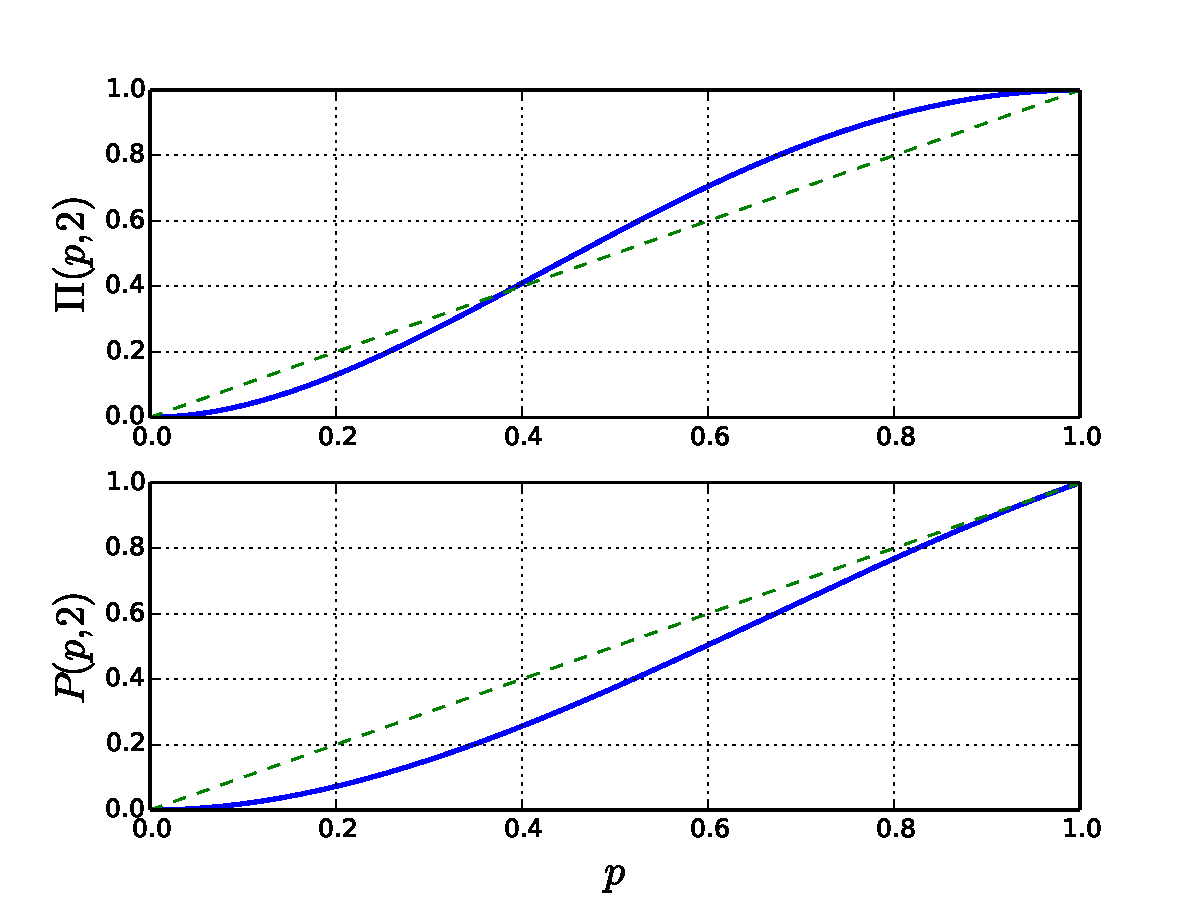
\includegraphics[width=\textwidth]{11.pdf}
\end{figure}

\newpage
We note some things about the curves: Both curves start at $0$ for $p=0$ and go to $1$ as $p\to 1$, this is very intuitive. They are also completely smooth. Note that the spanning cluster density is always below $p$, this makes perfect sense. The spanning cluster density is the probability of a random site to be a part of the spanning cluster. Now, the random site doesn't \emph{have} to be occupied, so the highest-estimate for $P$ should always be $p$---and occupied sites don't have to be part of a spanning cluster. In this case, if there \emph{is} a spanning cluster, all occupied sites automatically belong to it, so it is not surprising that the the difference from $p$ dies out as $\Pi\to 1$. For larger clusters however, it is very possible to have both a spanning cluster, and non-spanning cluster in the same experiment.

\subsection*{Measuring $\Pi(p,L)$ and $P(p, L)$ numerically}

For larger lattices, listing all the possible configurations becomes impossible due to the sheer number of them. Instead we do monte carlo simulations. By generating $N$ matrices of size $L$ and checking them against the probability $p$, we can look at the number of them that are percolating, the ratio of percolating systems to the total number of systems simulated gives an estimate for $\Pi(p,L)$ that improves as $N$ improves.

\clearpage

\section{ Cluster number density in 1-d percolation}
\begin{itemize}
	\item Define the cluster number density for 1-d percolation
	\item Show how it can be measured.
	\item Discuss the behavior when $p \to p_c$. How does it relate to your simulations in two-dimensional systems?
\end{itemize}

\subsubsection*{Definition of number cluster density}

In a random system, there will usually be very many different clusters of varying shapes and sizes. When $p > p_c$ there will usually be one or more spanning clusters, but also many non-spanning clusters. When $p < p_c$ there will usually just be many non-spanning clusters. We might ask the question how the sizes of the clusters are distributed, and how that distribution changes as $p \to p_c$. When $p\to p_c$ the clusters will tend to rapidly grow larger untill they become the system size and the system becomes percolating. The cluster number density $n(s,p)$ is part of this distribution

\paragraph{Definition} 
The cluster number density is the probability for a random site in the matrix to be a specific site in a cluster of size $s$.

The normalization requirement on the number cluster density is
$$P + \sum_s s n(s,p) = p,$$
In 1D, $p_c = 1$ so $P = 0$ when $p<p_c$ and we get
$$\sum_s s n(s,p) = (1-p)^2 p \sum_s s p^{s-1} =  (1-p^2) \frac{\d}{\d p} \sum_s p^s = (1-p^2) p \frac{\d}{\d p} (1-p^2)^{-1} = p.$$


The probability for a random site to be part of a cluster of size $s$ is then $sn(s,p)$, since any cluster of size $s$ has $s$ specific sites. In 1D, for a site to be the left-most site in a cluster of size $L$ is given by the fact that we need $p$ occupied sites and 2 non-occupied sites surrounding those $s$ sites.
$$n(s,p) = p^s (1-p)^2.$$
because a random site has a probability $p$ to be occupied, and then it is either part of the spanning cluster, or of a non-spanning cluster of size $s$. 

\subsubsection*{Characteristic cluster size}
To get a better understangin of $n(s,p)$, let us consider $p$ to be a constant. And look at the $s$-dependance of $n(s,p)$. In this case, $(1-p)^2$ is basicly just a normalization constant, and of no interest, so we look at only 
$$G(s) = n(s,p)(1-p)^{-2} = p^s.$$
If we plot a log-log plot of this function against $s$, we get 
\begin{figure}[ht]
\centering
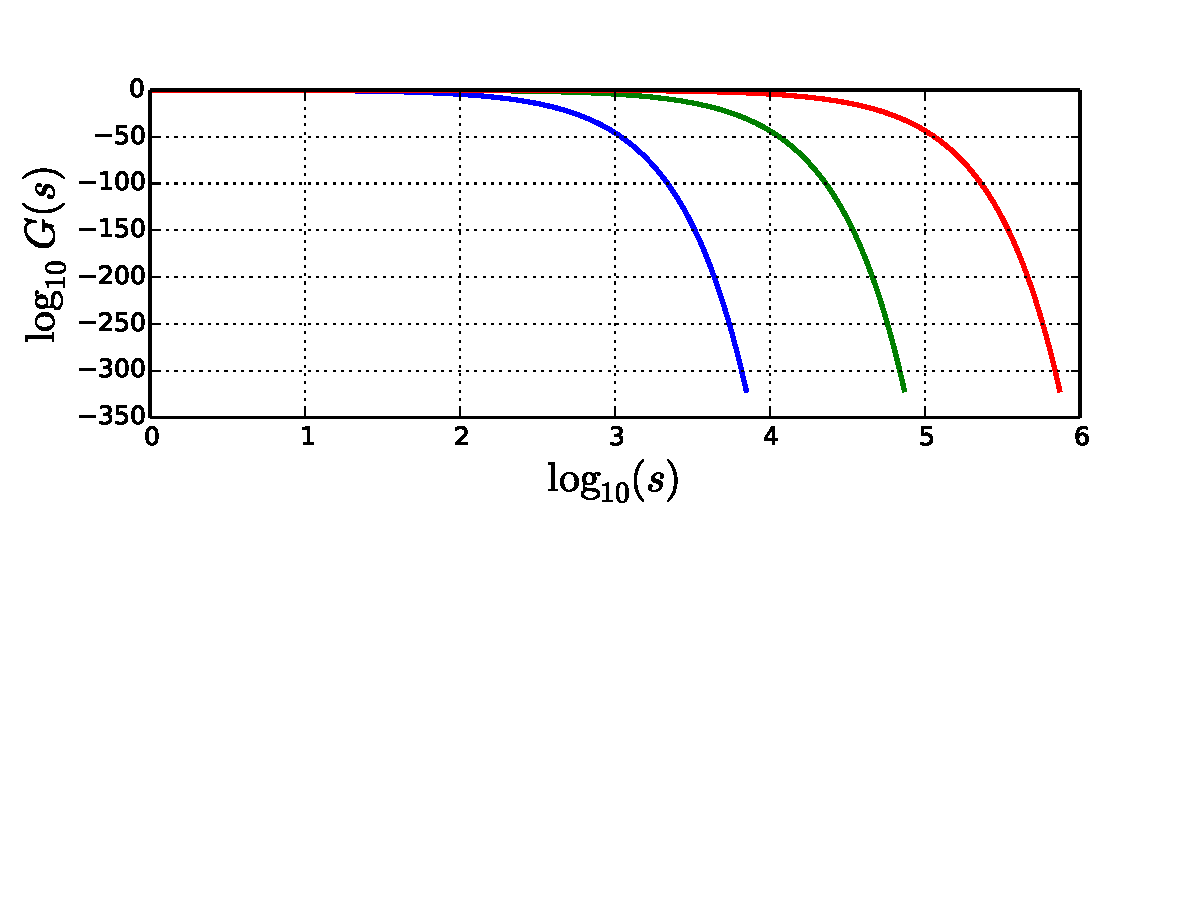
\includegraphics[width=\textwidth]{12.pdf}
\end{figure}
To understand this function we rewrite $G$ as follows
$$G(s) = p^s = e^{s \ln p} = e^{-s/s_\xi}, \qquad s_\xi \equiv -\frac{1}{\ln p}.$$
Where $s_\xi$ is the cut-off cluster size, also referred to as the characteristic cluster size. It is a cut-off, as 
$$G(s) = e^{-s/s_\xi} = \begin{cases}
1 & s \ll s_\xi, \\
0 & s \gg s_\xi, \\
\end{cases},$$
so when $s\to s_\xi$, $G$ (and thereby $n(s,p)$) starts decay exponentially.

\subsubsection*{Dependence on $p$}
We see that the $p$-dependence enters as $p$ affects how large the characteristic cluster size is
$$s_\xi = -\frac{1}{\ln p},$$
from this, we see that $s_\xi$ grows with $p$ (in 1D), which is very intuitive. As $p\to p_c (= 1)$ we can Taylor-expand
$$-\frac{1}{\ln p} = -\frac{1}{\ln(1 - (1 - p))} \simeq \frac{1}{1-p}.$$
And as $1 = p_c$ we get
$$s_\xi \simeq \frac{1}{p_c-p} = |p-p_c|^{-1/\sigma}.$$
Which is the general form of $s_\xi$ in \emph{any} dimension. In 1D, $\sigma = 1$.

So as $p\to p_c$, $s_\xi$ diverges as a power law.

\paragraph{Data collapse:} As the only $p$-dependence of $n(s,p)$ enters through $s_\xi$, we expect a data collapse if we instead plot $G$ as a function of $s/s_\xi$. To include the normalization $(1-p)^2$ we use the Taylor expansion, so that $(1-p)^2 \simeq s_\xi^{-2}$. So that we get
$$n(s,p) = s^{-\tau} F\bigg(\frac{s}{s_\xi}\bigg).$$

\subsubsection*{Numerical simulation}

We can generate a system with threshold $p$, and then count the number of clusters of size $s$: $N_s$ (the spanning cluster should not be included!). We can then estimate the cluster number density from
$$\bar{n(s,p)} = \frac{N_S}{L^d}.$$
A better estimate would of course be given by doing many experiments
$$\bar{n(s,p)} = \frac{N_S(M)}{ML^d}.$$
To do the counting $N_S(M)$ in a meaningful manner, we should use logarithmic binning as we have a fat tail.

\clearpage

\section{Correlation length in 1-d percolation}
\begin{itemize}
	\item Define the correlation length $\xi$ for 1-d percolation.
	\item Discuss its behavior when $p \to p_c$. 
	\item How is it related to cluster geometry and your results for twodimensional percolation?	
\end{itemize}

\subsubsection*{Correlation length $\xi$}

The characteristic cluster size $s_\xi$ says something about the size/mass/area of a cluster. The correlation length however, is used to characterize the extent of a cluster. We first define the correlation function $g(r)$, which is the probability of two occupied sites being a distance $r$ apart of begin connected---the $r$ coordinate is an integer denoting the number sites in between. In 1D, this is quite simple to compute, it is simply
$$g(r) = p^r = e^{r \ln p} = e^{-r/\xi}.$$
This function is quite flat for low $r$, but as $r\to \xi$ it starts decaying exponentially. As $\p \to p_c$ the correlation length diverges. We use the fact that $\p \to 1$ to Taylor expand
$$\ln p \simeq - (1-p)$$
so we have
$$\xi = \xi_0 (p_c - p)^{-\nu}.$$
Where $\xi_0$ and $\nu$ depends on the system, such as dimensionality etc. We note that $\xi$ diverges as a power law as $p \to p_c$.

\subsubsection*{Cluster geometry}

Now, the characteristic length says something about the extent of the cluster, but what about it's geometry? We can define a variance for the geometry of the cluster, such a quantitiy is known as the \emph{radius of gyration}. We define it as
$$R_i^2 = \frac{1}{s_i}\sum_{n=1}^{s_i} (\vec{r}_i - \vec{R}_i)^2.$$
Where $R_i$ is the radius of gyration for a given cluster $i$, $s_i$ is the cluster size, $n$ is a site label, $\vec{r}$ is the site location and $\vec{R}_i$ is the clusters centre of mass.

\subsubsection*{2D percolation}
For 1D, the extent and mass of a cluster is the same thing (a cluster can't be hollow), so 
$s_\xi = \xi,$
however, in higher dimensions
$$s_\xi \propto \xi^D, \qquad \mbox{where } D \mbox{ is a dimensionality constant } D < d.$$


An intersting use for $\xi$ is that it tells us when a finite system size will be a good approximation to an infite lattice. As we have done numerical modeling of a 2D lattice (it is not analytically solvable), we must neccesarily have a finite $L$, which might affect our results dramatically. However, if $\xi \ll L$, there should be no clusters of extent close to the lattice size, as the clusters of size larger than $\xi$ are exponentially surpressed. However, if $\xi \gg L$ there's a high probability of clusters the size of the system, and so the finite system size will definitely affect the results. As $\xi$ diverges as $p\to p_c$, a finite system size $L$ will never be a truely good approximation to the infite cluster as $p \to p_c$. 

We have
\begin{align*}
s_\xi \propto |p-p_c|^{-1/\sigma}, \\
s_\xi \propto \xi^D = |p-p_c|^{-D\nu},
D\nu\sigma = 1.
\end{align*}


\textbf{Finite Size Scaling}



\clearpage

\section{Cluster size in 1-d percolation}
\begin{itemize}
	\item Introduce the characteristic cluster size for the 1-d percolation problem.
	\item Discuss their behavior when $p \to p_c$.
	\item Relate to your simuluations on 2-d percolation.
\end{itemize}

\clearpage

\section{Measurement and behavior of $P(p, L)$ and $\Pi(p, L)$}
\begin{itemize}
\item Discuss the behavior of $P(p, L)$ and $\Pi(p, L)$ in a system with a finite system
size $L$.
\item How do you measure these quantities?
\end{itemize}

\subsubsection*{Behaviour}
\subsubsection*{Measurement}


 

\clearpage

\section{The cluster number density}
Introduce the cluster number density and its applications: 
\begin{itemize}
	\item Definition
	\item Measurement
	\item Scaling
	\item Data-collapse
\end{itemize}

\clearpage

\section{ Finite size scaling of $\Pi(p, L)$}
Discuss the behavior of $\Pi(p, L)$ in a system with a finite system size $L$. How
can we use this to find the scaling exponent $\nu$, and the percolation threshold, $p_c$?

\clearpage

\section{ Subsets of the spanning cluster}
Introduce and discuss the scaling of subsets of the spanning cluster. How can
we measure the singly-connected bonds, and how does it scale?

\clearpage

\section{ Random walks / Flow in a disordered system}
\begin{itemize}
	\item[Either:] Discuss the scaling theory for the distance $r^2(t)$ of a random walker
dropped at a random occopied site on either (1) the percolation system or (2)
the spanning cluster. (You can choose which case to discuss). Relate the results
to diffusion in a bulk fluid and in a nanoporous system.
\item[Or: ] How do you measure the conductivity of the spanning cluster? Discuss the
scaling theory for the conductivity $\sigma(p, L)$
\end{itemize}

\clearpage

\section*{Appendix}

\subsubsection*{Box-Muller transform}

The Box-Muller transform is a way to convert randomly drawn numbers from $[0,1)$ to standard normally distributed numbers. There are two versions of the Box-Muller transform, the basic and the polar. Both versions draw to independant uniformely random numbers, $u$ and $v$ from $(0,1)$ and generate two normal numbers at once using trigonometric functions. The difference is that the polar form implements rejection sampling. If the random numbers $u$ and $v$ are such $u^2 + v^2 \geq 1$, we reject the pair and draw two new ones. Initially this seems inefficient, (we need roughly 1.3 input numbers per output number) but the computation from $u$ and $v$ to normal numbers is computationally cheaper and for most modern computers trigonometric functions are much more expensive than drawing rand numbers.

\section*{Questions}

Are the signs in Darcy's Law as given in project 2 opposite? Look at wikipedia. Why would the volume flux be \emph{opposite} of the applied force? The law now says that flow goes \emph{against} the pressure gradient (from low pressure to high pressure).


% \section*{Laws of Thermodynamics}

% \subsubsection*{First law}
% The first law is a statement about conservation of energy. If we let $U$ denote the internal energy of a system, we state that we can decompose this energy change as \emph{heat}, $Q$ and \emph{work}, $W$.
% $$\Delta U = Q \pm W.$$
% Note that we use $\pm$ to denote the work, this is because we can define the work both \emph{on} the system or \emph{by} the system, both conventions are used regurarly and so care should be taken. The heat is usually defined as the heat \emph{entering} the system.

% If the number of particles in a system is constant the instantaneous work done by the system will be 
% $$\d W = P \d V,$$
% so we have
% $$\d U = \d Q - P \d V.$$

% \subsection*{Second law}
% The second law states that the entropy of an isolated system always will increase. Mathematically we can state it as
% $$\Delta S \geq T\Delta Q,$$
% at least for a constant temperature. For a reversible process, this becomes an equality
% $$\Delta S = T \Delta Q \quad \mbox{(reversible process)} $$
% This implies that a reversible process is a process that produces no entropy, it is thus a system continously changing through equilibria states and will therefore often be 
% infinitely slow. A reversible process is thus ususally an abstraction, and not a real quality of a process. Processes can however, be close to reversible.

% Combining the first and second law gives us the important inequality
% $$T\Delta S \geq \Delta U + P\Delta V.$$
% For an infinitesimal quantity, this will always be true
% $$T\ \d S = \d U + P\ \d V.$$

% \section*{Derivatives of state variables}
% From the equation
% $$\d U = T\ \d S - P\ \d V + \mu\ \d N,$$
% we get the derivatives
% \begin{align*}
% \b(\frac{\p S}{\p U}\b)_{V,N}=\frac{1}{T}, \qquad \b(\frac{\p S}{\p V}\b)_{U,N}=\frac{P}{V}, \qquad \b(\frac{\p S}{\p N}\b)_{U,V}=-\frac{\mu}{T}.
% \end{align*}

% \clearpage

% \section*{Maxwell relations}
% From the first law we have
% \beq \d U = T\ \d S - P\ \d V. \eeq \label{eq:maxwell1}
% Should therefore express $U$ as a function of $S$ and $V$, $U = U(S,V)$, can then look at the total derivative of $U$
% \beq \d U = \bigg(\frac{\p U}{\p S}\bigg)_V \d S + \bigg(\frac{\p U}{\p V}\bigg)_S \d V. \eeq \label{eq:maxwell2}
% Comparing \ref{eq:maxwell1} and \ref{eq:maxwell2} gives
% $$T = \bigg(\frac{\p U}{\p S}\bigg)_V, \qquad P = -\bigg(\frac{\p U}{\p V}\bigg)_S.$$

% Generally
% $$\frac{\p^2 U}{\p V \p S} = \frac{\p^2 U}{\p S \p V}.$$
% So we get
% $$\bigg(\frac{\p T}{\p V}\bigg)_S = -\bigg(\frac{\p P}{\p S}\bigg)_V.$$

% \subsubsection*{General state variables}
% Let us say we have three state variables, $X$, $Y$, $Z$, and we have an equation of state $Z(X,Y)$. We see that $Z$ is not a free variable, but is given by $X$ and $Y$. Of course, we could have said that $X$ is not the free variable, because it can be given by $X(Y,Z)$, i.e., the equation of state can be solved for any of the three state variables.

% The total derivatives of all equation of states become
% \begin{align*}
% \d Z = \bigg(\frac{\p Z}{\p X}\bigg)_Y \d X + \bigg(\frac{\p Z}{\p Y}\bigg)_X \d Y, \\
% \d X = \bigg(\frac{\p X}{\p Y}\bigg)_Z \d Y + \bigg(\frac{\p X}{\p Z}\bigg)_Y \d Z, \\
% \d Y = \bigg(\frac{\p Y}{\p X}\bigg)_Z \d X + \bigg(\frac{\p Y}{\p Z}\bigg)_X \d Z.
% \end{align*}
% Inserting $\d Y$ into $\d X$ gives
% $$\bigg[\bigg(\frac{\p X}{\p Y}\bigg)_Z\bigg(\frac{\p Y}{\p X}\bigg)_Z - 1\bigg]\d X  + \bigg[\bigg(\frac{\p X}{\p Y}\bigg)_Z\bigg(\frac{\p Y}{\p Z}\bigg)_X + \bigg(\frac{\p X}{\p Z}\bigg)_Y\bigg]\d Z = 0.$$
% The differentials are of course independant, so we get
% $$\bigg(\frac{\p X}{\p Y}\bigg)_Z = \bigg(\frac{\p Y}{\p X}\bigg)_Z^{-1},$$
% and
% $$\bigg(\frac{\p X}{\p Y}\bigg)_Z \bigg(\frac{\p Y}{\p Z}\bigg)_X \bigg(\frac{\p Z}{\p X}\bigg)_Y = -1.$$

% We can now let another state variable be given by $X$ and $Y$
% $$\d U = \bigg(\frac{\p U}{\p X}\bigg)_Y \d X + \bigg(\frac{\p U}{\p Y}\bigg)_X \d Y.$$
% Dividing by $\d X$ and holding the equation constant at $Z$ gives
% $$\b( \frac{\p U}{\p X} \b)_Z = \bigg(\frac{\p U}{\p X}\b)_Y + \b(\frac{\p U}{\p Y}\b)_X \b(\frac{\p Y}{\p X}\b)_Z$$

% \subsection*{Specific Heat}
% When we add a small amount of heat to a system, the temprature will rise by some small amount, this is the definition of the specific heat of that system. For a given state variable $X$ it is defined as
% $$C_X = \lim_{\Delta T \to 0} \b(\frac{\Delta Q}{\Delta T}\b)_X = T \b(\frac{\p S}{\p T}\b)_X.$$

% Starting at the first law we have
% $$T \d S = \d U + P\ \d V,$$
% inserting the complete derivative for $\d U$ gives
% $$T \d S = \b(\frac{\p U}{\p T}\b)_V \d T + \b(\frac{\p U}{\p V}\b)_T \d V + P\ \d V,$$
% If we look at the specific heat for a constant volume, we get
% $$C_V = \b(\frac{\p U}{\p T}\b)_V.$$
% If we instead keep the pressure constant, we get
% $$C_P = C_V + \b[\b(\frac{\p U}{\p V}\b)_T + P\b]\ \b(\frac{\p V}{\p T}\b)_P.$$
% This can also be formulated as
% $$C_P = \b(\frac{\p H}{\p T}\b)_P.$$
% Where $H$ is the \emph{enthalpy}:
% $$H = U + PV.$$

% \section*{Equation of State}
% For most systems all state variables are not independent, but will depend on each other. If we can explicitly give a state variable in terms of the other state variables, that is an equation of state. An example could be the relation $$P(T,V).$$
 
% The equation of state give important information about how matter will behave under different physical conditions and so is very material dependant.

% \subsection*{Ideal gas law}
% The ideal gas law is an equation of state
% $$P = \frac{NkT}{V}, \qquad P = kT\rho.$$

% \subsection*{Van der Waals Equation of State}
% The ideal gas presupposes no interaction between the particles. The van der Waals equation of state tries to include some interaction in a basic and approximate manner
% $$P = \frac{NkT}{V - Nb} - \frac{aN^2}{V^2}.$$
% Here $a$ and $b$ are parameters describing the particles, $b$ reflects the particles having some volume and $a$ models the attraction between the particles.

% \subsection*{Phase Transition}
% Two phases are in thermodynamic equilibrium, meaning the total entropy
% $$S(U,V,N) = S_1(U_1,V_1,N_1) + S_2(U_2,V_2,N_2),$$
% is maximized. Taking the total derivative
% \begin{align*}
% \d S &= \b(\frac{\p S_1}{\p U_1}\b)_{V_1, N_1} \d U_1 + \b(\frac{\p S_1}{\p V_1}\b)_{U_1, N_1} \d V_1 + \b(\frac{\p S_1}{\p N_1}\b)_{U_1, V_1} \d N_1 \\
% &\qquad + \b(\frac{\p S_2}{\p U_2}\b)_{V_2, N_2} \d U_2 + \b(\frac{\p S_2}{\p V_2}\b)_{U_2, N_2} \d V_2 + \b(\frac{\p S_2}{\p N_2}\b)_{U_2, V_2} \d N_2 \\
% \end{align*}
% Now, using the fact that $\d U_1 = -\d U_2$ etc, we can simplify this to
% \begin{align*}
% \d S &= \b[\b(\frac{\p S_1}{\p U_1}\b)_{V_1, N_1} - \b(\frac{\p S_2}{\p U_2}\b)_{V_2, N_2} \b] \d U_1 \\
% &\qquad  + \b[\b(\frac{\p S_1}{\p V_1}\b)_{U_1, N_1} - \b(\frac{\p S_2}{\p V_2}\b)_{U_2, N_2}\b]\d V_1 \\
% &\qquad\qquad+ \b[\b(\frac{\p S_1}{\p N_1}\b)_{U_1, V_1} - \b(\frac{\p S_2}{\p N_2}\b)_{U_2, V_2} \b]\d N_1 \\
% \end{align*}

% \clearpage

% \section*{Ensambles}

% In a microcanonical ensamble, the energy of the system is held constant. All microstates with the given energy are possible and of equal probability. Also known as a $NVE$-ensamble as the number of particles, volume and energy are constant.

% From wikipedia:
% In simple terms, the microcanonical ensemble is defined by assigning an equal probability to every microstate whose energy falls within a range centered at E. All other microstates are given a probability of zero. Since the probabilities must add up to 1, the probability P is the inverse of the number of microstates W within the range of energy,
% $P = 1/W$,
% The range of energy is then reduced in width until it is infinitesimally narrow, still centered at E. In the limit of this process, the microcanonical ensemble is obtained.

% \clearpage

% \section*{Phase space}

% In general, a system of $N$ particles is described by the particles position and momenta in all dimensions, these evolve in time according to some dynamical equations of the system, so we have
% $$q_i = q_i(t, q_0, p_0), \qquad p_i = p_i(t,q_0,p_0).$$
% Where $(q_0, p_0)$ are the inital conditions of the system. For most systems, the evolution can only be found numerically. A problem then, is that the systems are often chaotic, and so the finite precision in the initial conditions limits our possible solutions.

% A goal is to find the average of some quantity over a long time
% $$\bar{A} = \frac{1}{T}\int_0^T A(q(t), p(t)) \ \d t.$$
% And we will have to include states corresponding to all the parts of phase space visited, however, this requires knowledge of the phase trajectory, which we generally don't have.

% A solution put forth by Gibbs is to instead look at phase space as filled by a liquid, the density in phase space is then given by $\rho = \rho(q,p)$ and the number of systems in a volume element $\Delta q \Delta p$ is the given by $\rho(q,p)\Delta q \Delta p$. The greater the density is in a region of phase space, the greater the probability is to find the system in that part of phase space. And so we can now average over the density of the entire phase space to find thermodynamic quantities.

% In quantum mechanics, due to the Heisenberg uncertainty principle, a given particle state has the volume
% $$\d\omega = \frac{\d^f q\  \d^f p}{(2\pi \hbar)^f}.$$

% We of course choose the density of phase space in a manner that it is normalized in the sense that
% $$\int \d \omega \rho(q,p) = 1.$$
% Ensamble averages are then found from
% $$\langle A \rangle = \int \rho(q,p) A(q,p) \ \d \omega.$$

% It cannot be proven generally that the time-average, and the ensamble-average found from the density of phase space are equal, and we are now finding the ensamble-average through derivation, but obviously the time-average in experiment. For some systems they can be shown to be equal, but in general we have to simply invoke the ergodic hypothesis that state they are equal.

% \subsection*{Liouville's Theorem}
% To derive the behaviour of the density of phase space we can use the fact that the density of phase space is goverened by Hamilton's equations for each point. Also, no system can make discontinious jumps in the dynamical variables $q$ and $p$, and cannot start/stop exisiting, meaning the equation of continuity applies to the density
% $$\frac{\p \rho}{\p t} + \nabla \cdot \vec{J} = 0.$$
% Where $\vec{J}$ is the current of system points, which can be expressed as $\vec{J} = \rho\vec{V}$, where $\vec{V}$ is the velocity vector $\vec{V} = (\dot{\vec{q}}, \dot{\vec{p}})$. Writing out the nabla operator, we see that we can use Poisson brackets to compactily write the equation of continuity
% $$\nabla \cdot \vec{J} = \sum_i \b( \frac{\p p}{\p q_i}\frac{\p H}{\p p_i} - \frac{\p H}{\p q_i}\frac{\p \rho}{\p p_i}\b).$$
% \subsubsection*{Equation of continuity}
% $$\frac{\p p}{\p t} + \{\rho, H\} = 0.$$

% Now, the phase space density is generally a time-dependant field, $\rho(q,p,t)$ and so the total derivative is
% $$\frac{\d }{\d t} \rho = \frac{\p \rho}{\p t} + \{\rho, H\},$$
% which we see from the equation of continuity is zero. This is Liouville's theorem. Stated in words it says that the local density of phase space remains constant as seen by an observer moving with a system point.

% If we then follow an initial volume element with a constant density, it will remain at a constant volume, but generally change shape as time evolves. 

% An important consequence of Liouville's theorem is that if $\rho$ is initially constant throughout phase space, meaning all microstates are equally likely. It will remain so as time evolves.

% Ergodicity means that the system will eventually visit all of the phase space that is covered by the ensemble, and for ergodic system Liouvilles theorem implies that every microstate is equally likely to be visited with time.



% \subsection*{Poisson Bracket}
% In canonical coordinates, the Poisson bracket takes the form
% $$\{f,g\} = \sum_{i=1}^N \b(\frac{\p f}{\p q_i}\frac{\p g}{\p p_i} - \frac{\p f}{\p p_i}\frac{\p g}{\p q_i}\b).$$
% It has the same role as the commutator has in quantum mechanics.

% Any functions, $f, g, h$ of phase space and time follows
% \begin{itemize}
% 	\item Anticommutativity: $\{f, g\} = - \{g, f\}$
% 	\item Distributivity: $\{f+g, h\} = \{f, h\} + \{g, h\}$
% 	\item Product rule: $\{fg, h\} = \{f, h\}g + f\{g, h\}$
% 	\item If $k$ is time-dependant, but constant over phase space, then $\{f,k\} = 0$.
% \end{itemize}
% For cannonical coordinates
% \begin{itemize}
% 	\item $\{q_i, q_j\} = 0$
% 	\item $\{p_i, p_j\} = 0$
% 	\item $\{p_i, q_j\} = \delta_{ij}$
% \end{itemize}

% Using the Poisson bracket, we can write Hamilton's equations as
% $$\dot{q} = \{q, H(q,p)\}, \qquad \dot{p} = \{p, H(q,p)\}.$$

% More generally, for \emph{any} function that is not explicitly dependant on time, but only $q$ and $p$
% $$\frac{d}{dt}f(q,p) = \{f, H\},$$
% if there is an explicit time-dependance we have
% $$\frac{d}{dt}f(q,p,t) = \{f, H\} + \frac{\p f}{\p t}.$$

% \clearpage

% \section*{Microcannonical ensamble}
% A microcannonical ensamble is completely isolated, and so has constant $NVE$. The fundamental assumption of statistical mechanics states that all microstates in a microcannonical ensamble are equally likely.

% \subsubsection*{Ergodic hypothesis}

% States that over long time periods, the time spent by a system in some region of phase space, i.e., in given microstates, with the same energy is proportional to the volume of that region. Stated simpler: All accesible microstates are equiprobable over long periods of time.

% \subsubsection*{Liouville's Theorem}

% States that for Hamiltonian systems, the local density of microstates following a particle path through phase space is constant as viewed by an observer moving with the ensamble. 

% ma
% where $D\rho/Dt$ is the material or total derivative, it gives the change in $\rho$ seen by a particle moving with the flow. 

% Lioville's theorem shows that flow in phase space is conservative and the microcannonical ensemble must be time independent. (If phase space is of uniform density, then it will stay so forever).

% Note that the ergodic hypothesis is one specific solution to the Liouville theorem equation, in fact, it is the simplest.

% \section*{Cannonical ensamble}

% A cannonical ensamble is in thermal contact with a reservoir with temperature $T$. It can therefore exchange energy $E$ with the reservoir, but has $NVT$ constant. 

% To derive the statistics of the cannonical ensamble, we can treat the system-reservoir pair as a microcannonical ensamble, meaning all microstates are equally likely. Let us now assume there is a infinitesimal exchange of energy beween the reservoir and the system, we know that
% $$\d S_{\rm R} = \frac{1}{T}(\d U_{\rm R} + P \d V_{\rm R} - \mu \d N_{\rm R}).$$
% We throw away the $\d V$ and $\d N$ terms, and so we have
% $$S_{\rm R}(s_2) - s_{\rm R}(s_1) = \frac{1}{T}[U_{\rm R}(s_2) - U_{\rm R}(s_1)] = -\frac{1}{T}[E(s_2) - E(s_1)].$$
% Giving
% $$\frac{P(s_2)}{P(s_1)} = \frac{e^{-E(s_2)/kT}}{e^{-E(s_1)/kT}}.$$
% Giving the \textbf{Boltzmann factor}
% $$e ^{-E(s)/kT}.$$
% To get an actual probability, we need the normalization constant, giving the \textbf{Boltzmann distribution}
% $$P(s) = \frac{1}{Z}e^{-E(s)/kT},$$
% where 
% $$Z = \sum_s e^{-E(s)/kT}.$$
% The partition function is a constant in the sense that it does not depend on the microstate $s$, but it does change with the temperature $T$. In the limit $kT \to 0$, we see that $Z \to 1$ as the only contributing state is the ground state as all other possible microstates become supressed. As $kT$ increases, $Z$ grows, as more microstates become available to the system. If we shift all energies by a constant factor of $E_0$, the partition function picks up a factor $e^{-E_0/kT}$, but it is inconsequential as it cancels out when calculating the probabilities $P(s)$.

% Using the Boltzmann distribution, we can find expectancies as
% $$\langle X \rangle = \sum_s X(s) P(s) = \frac{1}{Z} \sum_s X(s) e^{-\beta E(s)}.$$

% For the energy this can be written convieniently as
% $$\langle E \rangle = \frac{1}{Z}\sum_s E(s) e^{-\beta E(s)} = \frac{1}{Z} \sum_s \frac{\p}{\p \beta} e^{-\beta E(s)}.$$
% Giving
% $$\langle E \rangle = \frac{1}{Z}\frac{\p Z}{\p \beta}. $$
% Which can again be rewritten as
% $$\langle E \rangle = - \frac{\p }{\p \beta} \ln Z. $$

% For the energy squared, we get
% $$\langle E^2 \rangle = \frac{1}{Z}\frac{\p^2 Z}{\p \beta^2}.$$
% Which can be rewritten as
% $$\langle E^2 \rangle = \frac{\p^2}{\p \beta^2} \ln Z + \bigg[\frac{1}{Z} \frac{\p Z}{\p \beta}\bigg]^2 = \frac{\p^2}{\p \beta^2} \ln Z + \bigg[\frac{\p }{\p \beta}\ln Z \bigg]^2 = \frac{\p^2}{\p \beta^2} \ln Z  + \langle x \rangle^2.$$
% And so the variance is easily written as
% $$\langle \Delta E^2 \rangle = \langle E^2 \rangle - \langle E \rangle^2 = \frac{\p^2}{\p \beta^2} \ln Z.$$


% To find other quantitiez, we can calculate the Helmholtz free energy
% $$F = -kT \ln Z.$$
% Giving us
% $$S = -\bigg(\frac{\p F}{\p T}\bigg)_{V, N}, \qquad P = -\bigg(\frac{\p F}{\p V}\bigg)_{T, N}, \qquad \mu = \bigg(\frac{\p F}{\p N}\bigg)_{T, V}.$$

% \clearpage

% \section*{Other}
% $$e^x \simeq 1 + x, \qquad x \ll 1.$$

% $$\ln(1-x) \approx -x, \qquad x \ll 1.$$
% $$(1-x)^k \approx 1-kx, \qquad x \ll 1.$$


% $$e^{\hbar\omega/kT} \simeq 1 + \frac{\hbar \omega}{kT}, \qquad T \gg \hbar\omega/k.$$

% \subsubsection*{Stirling's approximation}
% Coarse
% $$\log n! = n \log n - n,$$
% Fine
% $$n! = \sqrt{2\pi n} n^n e^{-n}.$$

% \section*{Constants}

% \begin{center}
% \begin{tabular}{|c|c|}	
% \hline
% Boltzmann's constant & $k = 1.381\times10^{-23} \mbox{JK}^{-1}$ \\ \hline 
% Avogadro's Number & $N_{\rm A} = 6.023\times10^{23} \mbox{mol}^{-1}$ \\ \hline 
% $k\cdot N_{\rm A}$ & $R = 8.314 \mbox{JK}^{-1}\mbox{mol}^{-1}$ \\ \hline
% \end{tabular}
% \end{center}

% \clearpage

% \section*{Einstein Solid}

% The Einstein solid is an attempt to describe the vibrations of the atoms in a regular lattice, it is based on two fundamental assumptions
% \begin{itemize}
% 	\item Each atom in the lattice is an \emph{independant} 3D quantum harmonic oscialltor
% 	\item All atoms oscillate with the same common frequency (this is the big contrast with the Debye model) 
% \end{itemize}

% Assuming we are looking at a lattice containing $N$ atoms, the first assumptions tells us we have $3N$ degrees of freedom, as each atom can vibrate in three independant directions. Each oscillator will be occupied by certain number of phonons, which are the quanta in lattice vibrations as photons are the quanta in electromagnetic oscillations. Phonons are bosons with no chemical potential ($\mu = 0$) so the Bose-Einstein distribution predicts that the average number of phonons per oscillator will be
% $$\langle n \rangle = \frac{1}{e^{\hbar \omega/kT} - 1}.$$
% As each phonon carries the energy $\hbar \omega$, we find the average energy per oscillator to be
% $$\langle \eps \rangle = \frac{\hbar \omega}{e^{\hbar \omega/kT} - 1}.$$
% Summing over all the degrees of freedom of the system gives the total internal energy as
% $$U = \frac{3N\hbar \omega}{e^{\hbar \omega/kT} - 1}.$$
% We can now find the specific heat
% $$C_V = 3Nk \bigg(\frac{\hbar \omega}{kT}\bigg)^2 \frac{e^{\hbar \omega/kT}}{(e^{\hbar \omega/kT}-1)^2}.$$
% We now introduce the characteristic Einstein temperature $T_E = \hbar \omega/k$ and we simplify the expression for the specific heat in the limits $T \ll T_E$ and $T \gg T_E$
% $$C_V = \begin{cases}
% 	3Nk (\frac{\hbar\omega}{kT})^2 e^{-\hbar\omega/kT}, & T \ll T_E, \\
% 	3Nk, & T \gg T_E.
% \end{cases}$$
% When the temperautre is high, we recove the Dulong-Petit law that predicts a constant heat capacity in agreement with the equipartition principle. However, when $T\to 0$ we see that $C_V \to 0$ as required by the third law, however, it goes to zero expoentially, while experiment shows that it should go as $C_V \propto T^3$.

% \clearpage

% \section*{Debye Theory of Solids}

% Instead of treating every atom as an independant harmonic oscillator, we instead focus on the phonons and treat it as a `phonon gas in a box' (the box being the solid).  The energy of a phonon is 
% $$\eps_n = \hbar \omega_n = \hbar v k_n = \frac{\hbar \pi v}{L}n,$$
% where $n$ is the mode of the phonon and $v$ is the speed of sound in the solid. The phonons follow a Bose-Einstein distribution, so the average energy of phonons in mode $n$ is then 
% $$\langle \eps_n \rangle = \frac{\eps_n}{e^{\eps_n/kT} - 1}$$

% Unlike for a photon gas, there is a minimum wavelength the phonon can have (two times the lattice spacing) and thus a maximum mode. For a cubic box, it will be $N_{\rm max} = \sqrt[3]{N}$ and so the total energy of all the phonons in the solid is
% $$U = 3\sum_{n_x=1}^{\sqrt[3]{N}}\sum_{n_y=1}^{\sqrt[3]{N}}\sum_{n_z=1}^{\sqrt[3]{N}} \langle \eps_n \rangle.$$
% Where we have multiplied the result by three, since sound waves can have three independant polarizations.

% Assuming $L$ is macroscopic, the density of modes will be very high, and we can change the sums into an integral. The three sums is actually a sum over a cubic box in $N$-space, but it will be simpler to instead integrate over an eigth-sphere with the same volume. The volume of the box is $N$ and so the sphere needs to have a radius of
% $$n_{\rm max} = \bigg(\frac{6N}{\pi}\bigg)^{1/3}.$$
% The angular integral will give $\pi/2$, so the total energy can then be written as
% $$U = \frac{3\pi}{2} \int_{0}^{n_{\rm max}}  n^2 \langle \eps_n \rangle \ \d n.$$
% Inserting the average energy gives
% $$U = \frac{3\pi}{2} \int_{0}^{n_{\rm max}} \frac{\hbar \pi v}{L}n^3 \frac{1}{e^{\hbar \pi v n/LkT} - 1} \ \d n.$$ 
% We now do the substitution $x \equiv \hbar \pi v n/LkT$.
% $$U = \frac{3\pi}{2} \frac{\hbar \pi v}{L} \bigg(\frac{LkT}{\hbar\pi v}\bigg)^4 \int_0^{x_{\rm max}} \frac{x^3}{e^x-1} \ \d x.$$
% Where 
% $$x_{\rm max} = \frac{\hbar\pi v}{LkT} \bigg(\frac{6N}{\pi}\bigg)^{1/3} \equiv \frac{T_D}{T},$$
% where we introudced the Debye temperature
% $$T_D = \frac{\hbar\pi v}{Lk} \bigg(\frac{6N}{\pi}\bigg)^{1/3}.$$
% We then have the total energy
% $$U = \frac{9NkT^4}{T_D^3}\int_0^{T/T_D} \frac{x^3}{e^x - 1} \ \d x.$$
% The integral can only be solved numerically. However, in the limits $T\ll T_D$ and $T \gg T_D$ we can simplify it.

% When $T\gg T_D$ the upper limit of the integral is much less than 1, and $x \ll 1$ so that $e^x \simeq 1 + x$. This gives
% $$U = \frac{9NkT^4}{T_D^3}\int_0^{T/T_D} x^2 \ \d x = \frac{9NkT^4}{T_D^3} \frac{T^3}{3T_D^3} = 3NkT.$$
% Which recovers the Dulong-Petit law
% $$C_V = 3Nk.$$

% When $T \ll T_D$, the upper limit is very large. The exponential in the denominator effectively kills the integrand when $x$ becomes large, so replacing the upper limit with $\infty$ introduces little error, giving
% $$U = \frac{9NkT^4}{T_D^3}\int_0^\infty x^2 \ \d x = \frac{9NkT^4}{T_D^3} \frac{\pi^4}{15} = \frac{3\pi^4}{5} \frac{NkT^4}{T_D^3}.$$
% Giving the heat capacity
% $$C_V = \frac{12\pi^4}{5}\bigg(\frac{T}{T_D}\bigg)^3Nk.$$
% Which gives us the Debye $T^3$ law.

% At $T = T_D$ the heat capacity has reached $95$ \% of it's maximum value, so as long as $T > T_D$ we can use the equipartition theorem without much trouble. Altough the Debye temperature can be calculated from speed of sound in a solid using the defintion, it is more common to choose the $T_D$ that makes the theoretical prediction best fit the measured heat capacity.

% \clearpage

% \section*{Bose-Einstein Condensation}

% We now turn to gases of bosons where the chemical potential is \emph{not} zero. Considering the system as $T \to 0$, we know that more and more particles will settle into the ground state. Looking at a boson gas in a $L^3$ box, the ground state will have energy
% $$\eps_0 = \frac{p^2}{2m} = \frac{\hbar^2k_0^2}{2m} = \frac{\hbar^2 \pi^2}{2mL^2}(1+1+1) = \frac{3\hbar^2 \pi^2}{2mL^2}.$$
% At any temperature, the system follows the Bose-Einstein distibution, so the number of particles in the ground state will be
% $$N_0 = \frac{1}{e^{(\eps_0 - \mu)/kT} - 1}.$$
% So we see that $\mu < \eps_0$ and $\mu \to \eps_0$ when $T\to 0$. In this limit, we can simplify the exponential
% $$N_0 = \frac{kT}{\eps_0 - \mu}.$$
% Now, we would be finished if we only knew $\mu$ as a function of $T$, but we don't. However, we do have a condition that can determine it
% $$\sum_s \frac{1}{e^{\eps_s -\mu/kT} - 1} = N.$$
% To use this condition, we transform it into an integral, this is valid when $kT \gg \eps_0$ so that the density of modes is high. Using the density of states
% $$g(\eps) = \frac{2}{\sqrt{\pi}}\bigg(\frac{m}{2\pi\hbar^2}\bigg)^{3/2} V \sqrt{\eps}.$$
% It is half that of the electron gas, as the electron gas has two spin orientations.
% $$N = \int_0^\infty g(\eps) \frac{1}{e^{(\eps-\mu)/kT}-1}\ \d \eps.$$

% If we assume that $\mu = 0$ we get
% $$N = 2.612\bigg(\frac{m kT}{2\pi \hbar^2}\bigg)^{3/2}V.$$
% Which can only be true for a single temperature $T$, we call this temperature $T_C$
% $$kT_c = 0.527 \frac{2\pi \hbar^2}{m}\bigg(\frac{N}{V}\bigg)^{2/3}.$$
% For temperatures $T>T_C$, we find $\mu < 0$, while for $T<T_C$ we find
% $$N_{\rm excited} = 2.612 \bigg(\frac{mkT}{2\pi\hbar^2}\bigg)^{3/2}V = N\bigg(\frac{T}{T_C}\bigg)^{3/2}, \qquad (T < T_C).$$

% \clearpage

% \section*{Thermodynamic potentials}

% To create a system from vacuum, we would need to suply the systems internal energy $U$. However, to make room for it in the environment, we also need to provide the work $PV$, where $P$ is the (constant) pressure of the environment, and $V$ is the total volume of the system. We define the \emph{enthalpy} to be 
% $$H \equiv U + PV.$$
% However, since the system will have some entropy $S$, it can absorb some energy from it's surrounding as heat to bring it to the same temperature. If the environment is at constant temperature $T$, the system will get the energy $TS$ for free, so the energy of the system is best described by \emph{Helmholtz' free energy}
% $$F \equiv U - TS.$$
% If we also include the $PV$-term, i.e., the cost of making room for the system, we have \emph{Gibb's free energy}
% $$G \equiv U - TS + PV.$$
% So we see that $G = F + PV = H - TS$. We can summarize the results as follows
% \begin{center}
% 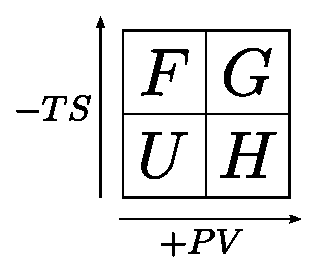
\includegraphics[width=0.3\textwidth]{potentials}
% \end{center}

% Now, in an isolated system, we know that the entropy always increases and will be maximized over long time scales. However, if we look at a system that is not isolated, but is in contact with a heat bath at constant temperature, the Helmholtz free energy of that system will be minimized. This is because the entropy of the system and reservoir combined will be maximized. Looking at the expression for the free energy $F = U - TS$, we see that the entropy of the system counts negative as expected, while the energy is positive. This is because the system will introduce entropy in the reservoir if it gives up energy to it, this is especially true at low temperatures $T$ as the entropy change per unit energy is proportional to $\frac{1}{T}$. Likewise, the Gibb's free energy is minimized for a system that has constant pressure and temperature, but can change volume and energy by interacting with it's environment
% \begin{itemize}
% 	\item At constant energy and volume (isolated system) entropy increases.
% 	\item At constant volume and temperature Helmholtz' free energy decreases.
% 	\item At constant pressure and temperature Gibb's free energy decreases.
% \end{itemize}
% In all three cases we assume that $N$ is held constant. So that $NVE \to S\uparrow$, $NVT \to F\downarrow$, $NPT\to G\downarrow$. If we want to include material contact, we use the \emph{grand free energy}: $\Phi \equiv U - TS - \mu N$.

% \newpage

% \subsubsection*{Thermodynamic identities}
% (Write out the total differential, and then substitute in for $\d U$.)
% \begin{align*}
% \d U &= T\ \d S - P \ \d V + \mu \ \d N, \\
% \d H &= T \ \d S + V\ \d P + \mu \ \d N, \\
% \d F &=  - S \ \d T - P \ \d V + \mu \ \d N, \\
% \d G &= -S \ \d T + V\ \d P + \mu \ \d N.
% \end{align*}

% From these we find many importan partial derivatives, for example
% $$S = -\bigg(\frac{\p F}{\p T}\bigg)_{V, N}, \qquad P = -\bigg(\frac{\p F}{\p V}\bigg)_{T, N}, \qquad \mu = \bigg(\frac{\p F}{\p N}\bigg)_{T,V}$$
% $$S = -\bigg(\frac{\p G}{\p T}\bigg)_{P, N}, \qquad V = \bigg(\frac{\p G}{\p P}\bigg)_{T, N}, \qquad\quad \mu = \bigg(\frac{\p G}{\p N}\bigg)_{T,P}$$

% Here we assume there's only one kind of particle, is there are more we replace $\mu \ \d N$ with $\sum_i \mu_i \ \d N_i$.

% \clearpage

% \section{Phase Transition}

% We consider an isolated system of two phases in thermodynamic equilibrium, we know the total entropy will be maximized spontaneously
% $$S(U,V,N) = S_1(U_1,V_1,N_1) + S_2(U_2,V_2,N_2).$$
% Giving the total change in $S$ to be (in each partial derivative, the two free variables are held constant)
% $$\d S = \bigg[\frac{\p S_1}{\p U_1} - \frac{\p S_2}{\p U_2}\bigg]\ \d U_1 + \bigg[\frac{\p S_1}{\p V_1} - \frac{\p S_2}{\p V_2}\bigg]\ \d V_1 + \bigg[\frac{\p S_1}{\p N_1} - \frac{\p S_2}{\p N_2}\bigg]\ \d N_1.$$
% Now, if the system is at thermal equilbrium, we know that $\d S = 0$ is zero for any change in $U_1$, $V_1$ and $N_1$ independently, meaning all the coefficients have to be independant. Using the thermodynamic indentity we have
% $$\bigg(\frac{\p S}{\p U}\bigg)_{V, N} = \frac{1}{T}, \qquad \bigg(\frac{\p S}{\p V}\bigg)_{U, N} = \frac{P}{T}, \qquad \bigg(\frac{\p S}{\p N}\bigg)_{U, V} = -\frac{\mu}{T}.$$
% So we see that the equilbrium conditions are
% $$T_1 = T_2, \qquad P_1 = P_2, \qquad \mu_1 = \mu_2.$$

% \subsection*{Clausius-Clapeyron}
% We now consider the slope of the phase boundary between two co-existing phases. If we want to move along the curve, we will generally have to change the pressure and temperature in the right way in relation to each other, so that $\d P$ and $\d T$. The equilibrium condition then gives
% $$G_g = G_l \quad \To \quad -S_g \ \d T + v_g \ \d P = - S_l \ \d T + v_l \ \d P.$$
% Which gives the slope
% $$\bigg(\frac{\d P}{\d T}\bigg) = \frac{S_g - S_l}{V_g - V_l} = \frac{L}{T\Delta V}.$$
% Where $L$ is the \emph{latent heat}. Note that $L$ and $\Delta V$ are both extensive, so the slope of the phase boundary must be an intensive quantity.

% \section*{Entropy}
% Entropy is given by
% $$S = k \log \Omega.$$
% Where $\Omega$ is the multiplicity, i.e., the number of microstates the system can inhabit.

% For substances with $S_0 = 0$ (Sometimes referred to as the third law, but is not universally true), we can find $S(T)$ as
% $$S(T) = \int_0^T \frac{C_{P}(T)}{T} \ \d T,$$
% for this to be valid, we must have 
% $$\lim_{T \to 0} C_P(T) = 0.$$
% At phase transitions, we also have a finite, discontinious jumps, which will be proportional in size to the latent heats of the phase transistors. So just at above the boiling temperature for a substance, we can for example find the entropy as
% $$S(T_b) = S_s(0\to T_m) + \frac{\Lambda_m}{T_m} + S_l(T_m \to T_b) + \frac{\lambda_B}{T_b\lambda}.$$

% The Gibbs entropy formula states
% $$S = -k \sum_s P_s \ln P_s.$$
% It is valid for both the microcanonical and canonical ensambles.

% \clearpage

% \section*{Extensivity and Intensivit}
% \begin{itemize}
% 	\item \textbf{Extensive:} $V$, $N$, $S$, $H$, $U$, $F$, $G$ 
% 	\item \textbf{Intensive:} $T$, $P$, $\mu$, $\rho$
% \end{itemize}
% Extensive times intensive is extensive. Extensive divided by extensive is intensive. Extensive times extensive is neither. Extensive plus extensive is extensive and likewise for intensive, extensive plus intensive is \emph{not allowed}.

% \clearpage

% \section*{Third law of thermodynamics}
 
% The third law states that as $T \to 0$, the entropy must tend to some constant number $S(0) = S_0$. Sometimes the third law is formulated as $S\to0$, but this is not universially true, as there are some systems with a degenerated ground state. However, the specific heat capacity can be formulated as
% $$C_V = \bigg(\frac{\p U}{\p T}\bigg)_V = \bigg(\frac{\p U}{\p S}\bigg)_V\bigg(\frac{\p S}{\p T}\bigg)_V = T\bigg(\frac{\p S}{\p T}\bigg)_V = \bigg(\frac{\p S}{\p \ln T} \bigg)_V.$$
% And as $S \to \mbox{const}$ as $T \to 0$ and $\ln T \to \infty$, we see that $C_V \to 0$. (The same is true for $C_P$).

% We see that this must be the case from the fact that
% $$S_f - S(0) = \int_0^{T_{f}} \frac{C_V}{T} \ \d T.$$
% If $C_V$ does not go to zero as $T \to 0$ we see that the denominator causes the integral to diverge, and as $S(0)$ has to be finite, it would imply that $S_f$ diverges, which is clearly not the case.

% \clearpage

% \section*{Response Functions}

% Specific heats are just one example of response functions
% $$C_V = \bigg(\frac{\p U}{\p T}\bigg)_V, \qquad C_P = \bigg(\frac{\p H}{\p T}\bigg)_P.$$
% $$C_P = C_V + \bigg[P + \bigg(\frac{\p U}{\p V}\bigg)_T\bigg]\bigg(\frac{\p V}{\p T}\bigg)_P.$$

% $$C_X = \lim_{\Delta T \to 0} \bigg(\frac{\Delta Q}{\Delta T}\bigg)_X = T\bigg(\frac{\p S}{\p T}\bigg)_X.$$

% Other response functions are compressibilities
% $$K_X = -\frac{1}{V}\bigg(\frac{\p V}{\p V}\bigg)_X.$$
% And thermal expansion coefficient
% $$\alpha = \frac{1}{V}\bigg(\frac{\p V}{\p T}\bigg)_P.$$
% All these response functions are related and one can show that
% $$C_P - C_V = \frac{TV}{K_T}\alpha^2.$$
% $$K_T - K_S = \frac{TV}{C_P}\alpha^2.$$
% and
% $$\frac{C_P}{C_V} = \frac{K_T}{K_S}.$$
% For magnetic systems, the susceptibilities play the same roles as the compressbilities.

% \clearpage

% \section*{Fluctations}
% We find expectencies from the Boltzmann distribution from
% $$\langle X \rangle = \sum_s X(s) P(s) = \frac{1}{Z} \sum_s X(s) e^{-\beta E(s)}.$$
% This gives us
% $$\langle E \rangle = - \frac{\p }{\p \beta} \ln Z.$$
% And 
% $$\langle E^2 \rangle = \frac{\p^2}{\p \beta^2} \ln Z + \bigg[\frac{\p }{\p \beta}\ln Z \bigg]^2 = \frac{\p^2}{\p \beta^2} \ln Z  + \langle x \rangle^2.$$
% And so
% $$\langle \Delta E^2 \rangle = \frac{\p^2}{\p \beta^2} \ln Z.$$

% Heat capacity is given by
% $$C_V = \bigg(\frac{\p U}{\p T}\bigg)_V.$$
% And so from $\langle E \rangle$ we find
% $$C_V = -\frac{\p }{\p T} \frac{\p}{\p \beta} \ln Z = \frac{\p}{\p \beta} \frac{\p \beta}{\p T} \frac{\p}{\p \beta} \ln Z = \frac{1}{kT^2} \frac{\p^2}{\p \beta^2} \ln Z.$$
% Comparing $\langle \Delta E^2 \rangle$ to $C_V$ gives
% $$\langle \Delta E^2 \rangle = kT^2 C_V.$$
% Note that $C_V$ is proportional to $N$, so it follows that the energy fluctations of a system is proportional to the number of particles in that system. However, as the total energy is also proportional to $N$, i.e., $\langle E \rangle \propto N$, it follows that the \emph{relative} energy fluctuations of the system are inversely proportional to the square root of the number of particles:
% $$\frac{\sqrt{\langle \Delta E^2 \rangle}}{\langle E \rangle} \propto \frac{1}{\sqrt{N}}.$$

% If we look at a $NVT$ ensamble, the `constant temperature' is the temperature of the heat bath and so the system does actually have temperature fluctuations (in comparison, a $NVE$ ensamble has no fluctuation in energy). Assuming the system has an instantaenous energy fluctuation, it will lead to a temperautre change given by
% $$\Delta T  = \Delta E \bigg(\frac{\p T}{\p E}\bigg)_{N,V} = \frac{\Delta E}{C_V}.$$
% And so the mean square fluctuations in temperature will be
% $$\langle \Delta T \rangle = \frac{\langle \Delta E^2 \rangle}{C_V^2} = \frac{kT^2}{C_V}.$$
% So the mean square temperature fluctuations are inversely proportional to $N$. However, unlike the total energy, the temperature of the system is an intensive size
% and independent
% of $N$,
%  so the relative 
% temperature fluctuations will also be inversely proportional to the square root of the number of particles
% $$\frac{\sqrt{\Delta T^2}}{T} \propto \frac{1}{\sqrt{N}}.$$

% \clearpage

% \section*{Equipartition Theorem}

% The equipartition theorem states that any quadratic degree of freedom will carry an average energy of $kT/2$ when the system is in equilibirum. As an example, consider the ideal gas, which only has the kinetic energy of the gas particles (as the particles are non-interacting), the hamiltonian will be
% $$H = \sum_{i=1}^N \frac{1}{2}m({v_i}_x^2+{v_i}_y^2+{v_i}_z^2),$$
% and so the average kinetic energy of the ideal gas will be
% $$U = \frac{3}{2}NkT,$$
% at thermal equilibrium. Which leads to the law of Dulong-Petit that $C_V = 3Nk$ for an ideal gas.

% The equipartition theorem breaks down at low temperature as the discrete nature of energy levels, i.e, start to matter. The equipartition theorem only applies when in the high-temperature limit where the spacing between energy levels is much less than $kT$.

% \clearpage

% \section*{Random Walker}

% The symmetric walker is given by uncorrelated steps to the left and right with the same probability $p=q$ and often we start the particle in the origin $x_0 = 0$.
% $$x_N = \sum_{i=1}^n \delta x_i.$$
% We find the expectation as a difference equation, we have
% $$x_{i+1} = x_{i} + \delta x_i.$$
% Inserting for the step $\delta x_i$ gives
% $$x_{i+1} = \begin{cases}
% 	x_i + a & \mbox{with probability } p, \\
% 	x_i - a & \mbox{with probability } q,
% \end{cases}$$
% So we have
% $$\langle x_{i+1} \rangle = p(\langle x_i \rangle + a) + q(\langle x_i \rangle - a) = \langle x_i \rangle + (p-q)a.$$
% If $p=q=1/2$ we get
% $$\langle x_{i+1} \rangle = \langle x_i \rangle \quad \To \quad \langle x_n \rangle = x_0 = 0.$$

% Now we calculate the expectany of the square displacement, we have
% $$x_{i+1}^2 = x_{i}^2 + 2x_i\delta x_i + \delta x_i^2.$$
% Inserting for $\delta x_i$ gives
% $$x_{i+1}^2 = \begin{cases}
% 	x_i^2 + 2x_ia + a^2 & \mbox{with probability } p, \\
% 	x_i^2 - 2x_ia + a^2 & \mbox{with probability } q,
% \end{cases}$$
% so the expectancy becomes
% $$\langle x_{i+1}^2 \rangle = \langle x_i^2 \rangle 2(p-q)a \langle x_i \rangle + a^2.$$
% For the symmetric walker ($p=q$) we then get
% $$\langle x_{i+1}^2 \rangle = \langle x_i^2 \rangle + a^2 \quad \To \quad \langle x_n^2 \rangle = na^2.$$
% Which we can write as the linear diffusion
% $$\langle x \rangle(t) = 2Dt,$$
% for $D = a^2/\Delta t$.

% \clearpage

% \section*{Central Limit Theorem}

% Let $X$ be a stochastic variable that follows a distribution with a well-defined mean $\mu$ and finite variance $\sigma^2$. Then if take many indenpendant samples of $X$: $\langle x_i \rangle_{i=1}^{N}$. The central limit theorem states that as $N$ grows large, the sum of the samples $\sum_i x_i$ will follow a normal distribution. The distribution being sampled is often referred to as the \emph{parent distribution} and does not have to resemble a normal distribution.

% To be more specific, if we calculate the sample average
% $$\bar{X} = \frac{\sum_{i=1}^N X_i}{N}.$$
% Then $\bar{X}$ is also a stochastic variable. The expectancy of $\bar{X}$ will obviously be the mean $\mu$ by the law of large numbers. The CLT however, also guarantees that $\bar{X}$ will be (approximately) normal distributed with variance $\sigma^2/n$. If we instead of taking the sample average just take the sample sum, 
% $$S_n = \sum_{i=1}^N X_i,$$
% then the mean will be $N\mu$ and the variance will be $N\sigma^2$. If we want a $N(0, \sigma^2)$ distribution we can study $\sqrt{N}(S_n - \mu)$. And if we a standard normal distribution, we can study
% $$\frac{\sqrt{N}(S_n - \mu)}{\sigma}.$$

% \clearpage

% \section*{Langevin Equation}

% Ikke pensum?

% % We will now find the variance as a function of time analytically for the symmetric $p=1/2$ walker. For this walker, we now that the increment $x_i$ is positive with probability 1/2 and negative with probability $1/2$. So the position of the walker grows as
% % $$X_{i+1} = X_{i} \pm 1,$$
% % where the `$\pm$' refers to the different steps. From this, we easily find how the expectancy of the displacement grows
% % $$\langle X \rangle_{i+1} = \langle X \rangle_i + \frac{1}{2} - \frac{1}{2} = \langle X \rangle_i$$
% % So from the fact that $X_0 = 0$, we see that $\langle X \rangle_t = 0.$ By squaring the equation,
% % $$X_{i+1}^2 = X_{i}^2 \pm 2X_{i} + 1,$$
% % we can also find how the expectancy of the squared displacement grows
% % $$\langle X_{i+1}^2 \rangle = \langle X_{i}^2 \rangle + 1,$$
% % and so from $X^2_0 = 0$ we get $\langle X^2\rangle_t = t$.

% % The variance at time $t$ is then
% % $$\langle \Delta X^2 \rangle_t = \langle X^2 \rangle_t - \langle X \rangle_t^2 = t.$$
% % Which we may write as
% % $$\langle \Delta X^2 \rangle_t = 2Dt,$$
% % for $D=1/2$. 
% \clearpage

% \section*{Magnetic Systems}

% When looking at magnetic systems, the magnetic moment of particles can be aligned with or against a magnetic field, which will lead to work. This means the particle or system can perform work by changing their magnetization (or rather, the direction of their magnetization). We reflect this by changing the pressure-work to magnetic-work
% $$\d W = P\ \d V \quad \to \quad \d W = B\ \d M.$$
% Both $P$ and $M$ are intensive, while $V$ and $M$ are extensive, so this change makes sense. It follows that
% $$\d U = T\ \d S + B \ \d M.$$
% And from this identity we can derive many new partial derivatives
% $$T = \bigg(\frac{\p U}{\p S}\bigg)_M, \qquad B = \bigg(\frac{\p U}{\p M}\bigg)_S,$$
% we can also find new Maxwell relations.

% The enthalpy no changes to
% $$H(S, B) = U - BM.$$
% And the free energy becomes
% $$F(T, M) = U - TS.$$
% And so we get
% $$\d F = -S \ \d T + B\ \d M,$$
% giving
% $$S = -\bigg(\frac{\p F}{\p T}\bigg)_M, \qquad B = \bigg(\frac{\p F}{\p M}\bigg)_T,$$

% And similar for the Gibbs free energy
% $$G = U - BM - TS, \qquad \d G = - M\ \d B - S\ \d T.$$
% $$S = -\bigg(\frac{\p G}{\p T}\bigg)_B, \qquad M = \bigg(\frac{\p G}{\p B}\bigg)_T,$$

% The \emph{susceptibility} is the change in magnetization as a result of the change in field
% $$\chi = \bigg(\frac{\p M}{\p B}\bigg)_T.$$
% And we also define the spefific heat
% $$C_B = \bigg(\frac{\p H}{\p T}\bigg)_B.$$

% \subsection*{Magnetic materials}

% The interaction energy between a magnetic material and a magnetic field is given by $U_B = -MB$ and for weak fields, we can write the induced magnetic moment as $M = \chi B$. We divide materials into three classes. Diagmagnetic materials have negative susceptibilites, $\chi < 0$, and so the induced magnetic moment will increase the energy of the system, thus we must perform work to move the material into the magnetic field (diamagnetic materials are repelled by magnetic fields). Paramagnetic materials however, have positive susceptibilities, $\chi > 0$, and are thus attracted to magnetic fields. Paramagnetic materials that retain the induced magnetization even when removed from the external field are referred to as \emph{ferromagnetic}.

% \subsubsection*{Paramagnets}

% In an ideal paramagnet, every dipole will only react with the external magnetic field, and will not interact directly with it's closest neighbors. In most paramagnetic crystals, the interaction with neighboring atoms can be ignored without introducing to much error. Every dipole will then get an energy eigenvalues
% $$\eps_m = -g\mu_B B m, \quad m=-J, -J+1, \ldots, J-1, J.$$
% The partition function becomes
% $$Z = \sum_{m=-J}^J e^{\beta g\mu_B B M}.$$
% This is a geometric series and evaluates to
% $$Z = \frac{e^{(J+1)a} - e^{-aJ}}{e^a - 1} = \frac{\sinh \frac{2J+1}{2J}}{\sinh \frac{x}{2J}}.$$
% Where $x = \beta g \mu_B B J$. And from this the Gibbs free energy follows $G = -kT \log Z$, and so we find the expectency for the magnetization of a single dipole to be
% $$m = \langle \op{m}_z \rangle = -\frac{\p G}{\p B} = g\mu_B J B_J(x).$$
% Where Brillouin function
% $$B_J(x) = \frac{2J+1}{2J}\coth \frac{2J+1}{2J} x - \frac{1}{2J}\coth \frac{x}{2J}.$$
% For small values of $x$ it is approximately linear
% $$B_J(x) = \frac{J+1}{3J}x + \mathcal{O}(x^3).$$
% For large $x$, it approaches $1$ for all $J$. As the field gets strong, all dipoles align parallel to the field, so $\mu = g\mu_B J$
% For large spin we have
% $$B_J(x)\big|_{J\gg1} = L(x) = \coth x - \frac{1}{x},$$
% This is the Langevin function, it is the classical limit of magnetization.
% In the other limit, the minimum is $J=1/2$ and the Brillouin function simplifies to
% $$B_{\frac{1}{2}}(x) = 2\coth 2x - \coth x = \frac{1 + \coth^2 x}{\coth x} = \tanh x.$$

% With the exception of very small temperatures, we can use the linear approximation, this gives
% $$M = Nm = \frac{Ng^2\mu_B^2J(J+1)B}{3kT}.$$
% And the susceptiblity
% $$\chi = \frac{Ng^2\mu_b^2J(J+1)B}{3kT}.$$
% This is sometimes referred to as Curie's law, where 
% $$M = C \frac{B}{T}, \qquad \chi = \frac{C}{T}.$$

% \subsection*{Ferromagnetic materials}
% For high temperatures (much higher than the curie temperature $T_C$), a ferromagnetic material behaves as a paramagnetic one, as described by the Curie-Weiss law
% $$\chi = \frac{C}{T-T_C}.$$
% The big difference is there is a phase change at $T = T_C$ where the susceptibility diverges, at temperatures below the Curie temperature, the material spontaneously magnetize. Experiment shows that the susceptibility diverges like
% $$\chi \propto |T-T_C|^{-\gamma}.$$
% Where $\gamma = 1.4$. We also find that
% $$C_B \propto |T-T_C|^{-\alpha}.$$



% \subsection*{Interacting dipoles}

% However, in real materials, the orientation of a specific dipole will depend and affect the orientation of at least it's closest neighbors. A material where the magnetic dipoles tend to be oriented in the same direction is a \emph{ferromagnet}, this will lead to magnetic domains and the material can have a spontaneous magnetization even when there is no external magnetic field. A material where the dipoles tend to be oriented in the opposite direction of their neighbors is called a \emph{antiferromagnet}.

% A ferromagnet will have spontaneous magnetization at low temperatures, as the temperature increases, the magnetization reduces slowly. At the curie temperature there is a phase change and any total magnetization vanishes.

% \clearpage

% \section*{Ising model}

% We neglect any long range interaction between dipoles, and let only dipoles affect the closest dipoles. We focus on a single domain in a ferromagnet. (Note that the ising model is a very simple model, at low temperature the model fails, as it should describe the long-wavelength \emph{magnons}), however, at temperatures close to the Curie temperature, this simple model is remarkably good.

% We say that a neighboring pair of dipoles carry an energy $\eps$ if they are aligned the same way, and $-\eps$ if they are aligned oppositely. So we have
% $$U = - \eps \sum_{\mbox{neighboring pairs}} s_is_j.$$
% Calculating the partition function in 2D is very difficult as the number of system structures grows as $2^N$. 

% \subsection*{Exact solution in 1D}
% In 1D, each dipole only has two neighbors, so we can find the partition function exactly
% $$U = -\eps \sum_{i=1}^{N-1} s_i s_{i+1} = -\eps(s_1s_2 + s_2s_3 + \ldots s_{N-1}s_N).$$
% And so the partition function becomes
% $$Z = \sum_{s_1}\sum_{s_2}\cdots\sum_{s_N}e^{-\beta U(s_1,s_2,\ldots,s_N)} =  \sum_{s_1}\sum_{s_2}\cdots\sum_{s_N} e^{\beta \eps s_1s_2}e^{\beta \eps s_2s_3}\cdots e^{\beta \eps s_{N-1}s_{N}}.$$
% Where every sum is over $\pm 1$. Not that the last Boltzmann factor is the only one that depends on $s_N$, so we can pull all the other factors out of the $s_N$ sum, and we have
% $$Z = \sum_{s_1}\sum_{s_2}\cdots\sum_{s_N-1} e^{\beta \eps s_1s_2}e^{\beta \eps s_2s_3}\cdots e^{\beta \eps s_{N-2}s_{N-1}} \sum_{s_N} e^{\beta \eps s_{N-1}s_{N}}.$$
% And the final sum becomes
% $$\sum_{s_N} e^{\beta \eps s_{N-1}s_{N}} = e^{\beta \eps} + e^{-\beta \eps} = 2\cosh\beta \eps.$$
% We can now do the same for the $s_{N-1}$ sum, and get the same result. We do this all the way down to the $s_2$ sum and end up with
% $$Z = \sum_{s_1} \big(2\cosh \beta \eps \big)^{N-1}.$$
% The final sum only contributes a factor of 2, so we need to do an approximation
% $$Z = 2^N (\cosh \beta \eps)^{N-1} \approx (2 \cosh \beta \eps)^N.$$
% From this we get the energy
% $$U = -\frac{\p}{\p \beta} \ln Z = -N \frac{\sinh \beta \eps}{\cosh \beta \eps} \eps = - N\eps \tanh \beta \eps.$$
% Which goes to $-N\eps$ as $T\to 0$, i.e., all dipoles align as $T\to 0$ and $U \to 0$ as $T \to \infty$, i.e., all dipoles align randomly as high temperatures. (This is the same $Z$ and $U$ as for the paramagnet with $\eps = \mu B$, the difference is that the paramagnet makes all dipoles align along an external field, while the ising crystel just makes the dipoles align along their neighbors).

% The 1D exact solution has a smooth energy transistions and \emph{does not} give a critical temperature, to get the phase transistion we have to turn to the 2D ising model first solved by Onsager.

% \section*{Mean field theories}

% We now look at a single dipole with spin $s_i$, somewhere in the interior of the lattice. Let $n$ bethe number of nearest neighbors, we then have
% $$n = \begin{cases}
% 	2 & \mbox{in 1D}; \\
% 	4 & \mbox{in 2D (square lattice)}; \\
% 	6 & \mbox{in 3D (simple cubic lattice)}; \\
% 	8 & \mbox{in 3D (body-centered cubic lattice)}; \\
% 	12 & \mbox{in 3D (face-centered cubic lattice)}. \\
% \end{cases}$$
% We now assume that the neighbors have frozen spins, and so our only degree of freedom is $s_i$. If we let $j$ run over all the nearest neighbors of $s_i$ we get
% $$E_\up = -\eps \sum_{j} s_j = -\eps\bar{s}, \qquad E_\down = \eps \bar{s}.$$
% And so the partition function for the isolated dipole becomes
% $$Z_i = e^{\beta \eps n \bar{s}} + e^{-\beta \eps n \bar{s}} = 2\cosh{\beta\eps n\bar{s}}.$$
% And from this partition function we can calculate the expectancy of $s_i$, getting
% $$\langle s_i \rangle = \frac{1}{Z_i}\bigg[e^{\beta \eps n \bar{s}} - e^{-\beta \eps n \bar{s}} \bigg] = \frac{2\cosh{\beta\eps n\bar{s}}}{2\cosh{\beta\eps n\bar{s}}} = \tanh{\beta\eps n\bar{s}}.$$

% Now the \textbf{fundamental approximation of the mean field approximation} is that we assume $\bar{s_i} = \bar{s}$. This means we assume the average magnetization is uniform across the entire lattice, and so all spins `see' the same neighborhood. This gives the equation
% $$\bar{s} = \tanh{\beta\eps n\bar{s}}.$$
% And $\bar{s}$ now refers to the average magnetization dipole alignment across the entire lattice.

% This equation is transcendental and cannot be solved on closed form. If we plot it out graphically, we see that we have to major cases. If $\beta \eps n < 1$, which implies $kT > n\eps$, the slope of the hyperbolic tangent is so low that there is only one solution, at $\bar{s} = 0$, i.e., there is no net magnetization of the material. For $k T < n\eps$, there are three solutions, an unstable solution at $\bar{s} = 0$ and two stable ones, located symmetrically around the center. This means the system will acquire a net nonzero magnetization, which is equally likely to be positive or negative.

% We see that the critical temperature is the temperature where $kT_c = n\eps$, since this is when we go from having a single to three solutions. The critical temperature is thus proportional to both the coupling strength and the number of neighbors, no shock there. Note that the mean field approximation predicts a critical temperature even in 1D, which we did not find in our analytical answer---this is simply because the simple mean field approximation is terrible in 1D.



% \clearpage



% \section*{Van der Waals equation}


\end{document}



 
